% Options for packages loaded elsewhere
\PassOptionsToPackage{unicode}{hyperref}
\PassOptionsToPackage{hyphens}{url}
%
\documentclass[
]{book}
\title{Estadística}
\author{Alejandro Cáceres (\href{mailto:alejandro.caceres.dominguez@upc.edu}{\nolinkurl{alejandro.caceres.dominguez@upc.edu}})}
\date{2023-02-27}

\usepackage{amsmath,amssymb}
\usepackage{lmodern}
\usepackage{iftex}
\ifPDFTeX
  \usepackage[T1]{fontenc}
  \usepackage[utf8]{inputenc}
  \usepackage{textcomp} % provide euro and other symbols
\else % if luatex or xetex
  \usepackage{unicode-math}
  \defaultfontfeatures{Scale=MatchLowercase}
  \defaultfontfeatures[\rmfamily]{Ligatures=TeX,Scale=1}
\fi
% Use upquote if available, for straight quotes in verbatim environments
\IfFileExists{upquote.sty}{\usepackage{upquote}}{}
\IfFileExists{microtype.sty}{% use microtype if available
  \usepackage[]{microtype}
  \UseMicrotypeSet[protrusion]{basicmath} % disable protrusion for tt fonts
}{}
\makeatletter
\@ifundefined{KOMAClassName}{% if non-KOMA class
  \IfFileExists{parskip.sty}{%
    \usepackage{parskip}
  }{% else
    \setlength{\parindent}{0pt}
    \setlength{\parskip}{6pt plus 2pt minus 1pt}}
}{% if KOMA class
  \KOMAoptions{parskip=half}}
\makeatother
\usepackage{xcolor}
\IfFileExists{xurl.sty}{\usepackage{xurl}}{} % add URL line breaks if available
\IfFileExists{bookmark.sty}{\usepackage{bookmark}}{\usepackage{hyperref}}
\hypersetup{
  pdftitle={Estadística},
  pdfauthor={Alejandro Cáceres (alejandro.caceres.dominguez@upc.edu)},
  hidelinks,
  pdfcreator={LaTeX via pandoc}}
\urlstyle{same} % disable monospaced font for URLs
\usepackage{longtable,booktabs,array}
\usepackage{calc} % for calculating minipage widths
% Correct order of tables after \paragraph or \subparagraph
\usepackage{etoolbox}
\makeatletter
\patchcmd\longtable{\par}{\if@noskipsec\mbox{}\fi\par}{}{}
\makeatother
% Allow footnotes in longtable head/foot
\IfFileExists{footnotehyper.sty}{\usepackage{footnotehyper}}{\usepackage{footnote}}
\makesavenoteenv{longtable}
\usepackage{graphicx}
\makeatletter
\def\maxwidth{\ifdim\Gin@nat@width>\linewidth\linewidth\else\Gin@nat@width\fi}
\def\maxheight{\ifdim\Gin@nat@height>\textheight\textheight\else\Gin@nat@height\fi}
\makeatother
% Scale images if necessary, so that they will not overflow the page
% margins by default, and it is still possible to overwrite the defaults
% using explicit options in \includegraphics[width, height, ...]{}
\setkeys{Gin}{width=\maxwidth,height=\maxheight,keepaspectratio}
% Set default figure placement to htbp
\makeatletter
\def\fps@figure{htbp}
\makeatother
\setlength{\emergencystretch}{3em} % prevent overfull lines
\providecommand{\tightlist}{%
  \setlength{\itemsep}{0pt}\setlength{\parskip}{0pt}}
\setcounter{secnumdepth}{5}
\usepackage{booktabs}
\ifLuaTeX
  \usepackage{selnolig}  % disable illegal ligatures
\fi
\usepackage[]{natbib}
\bibliographystyle{plainnat}

\begin{document}
\maketitle

{
\setcounter{tocdepth}{1}
\tableofcontents
}
\hypertarget{objetivo}{%
\chapter{Objetivo}\label{objetivo}}

Este es el curso de introducción a la estadística de la EEBE (UPC).

La estadística es un \textbf{lenguaje} que permite afrontar problemas nuevos, sobre los que no tenemos solución, y en donde interviene la \textbf{aleatoridad}.

En este curso trataremos los \textbf{conceptos fundamentales} de estadística.

\begin{itemize}
\item
  3 horas de \textbf{teoría} por semana: Explicaremos los conceptos, haremos ejercicios.
\item
  6 horas de \textbf{estudio individual} por semana: Notas notas de curso y los recursos en ATENEA.
\item
  2 horas de Solución de problemas con \textbf{R}: Sesiones presenciales con ordenador (Prácticas).
\end{itemize}

Las fechas de exámenes y material de estudio adicional se pueden encontrar en \textbf{ATENEA metacurso}:

Objetivos de evaluación:

\textbf{Q1} (10\%): Prueba en ordenador duración 2h en las fechas indicadas.

\begin{enumerate}
\def\labelenumi{\alph{enumi}.}
\tightlist
\item
  Dominio de comandos básicos en R (Prácticas)
\item
  Capacidad de calcular estadísticos descriptivos y gráficos, en situaciones concretas (Teoría/Práctica)
\item
  Conocimiento sobre la regresión lineal (Prácticas)
\end{enumerate}

\textbf{EP1} (25\%): Prueba escrita (2-3 problemas)

\begin{enumerate}
\def\labelenumi{\alph{enumi}.}
\tightlist
\item
  Capacidad de interpretación de enunciados en fórmulas de probabilidad (Teoría).
\item
  Conocimiento de las herramientas básicas para solucionar problemas de probabilidad conjunta y probabilidad condicional (Teoría).
\item
  Dominio matemático de funciones de probabilidad para calcular sus propiedades básicas (Teoría).
\end{enumerate}

\textbf{Q2} (10\%): Prueba en ordenador duración 2h en las fechas indicadas

\begin{enumerate}
\def\labelenumi{\alph{enumi}.}
\tightlist
\item
  Capacidad de identificación de modelos de probabilidad en problemas concretos (Teoría/Práctica).
\item
  Uso de funciones de R para calcular probabilidades de modelos probabilísticos (Práctica/Teoría)
\end{enumerate}

\textbf{Q3} (10\%): Prueba en ordenador duración 2h en las fechas indicadas

\begin{enumerate}
\def\labelenumi{\alph{enumi}.}
\tightlist
\item
  Capacidad de identificación de un estadístico de muestreo y sus propiedades (Teoría/Práctica)
\item
  Conocimiento de cómo calcular la probabilidad de los estadísticos de muestreo (Teoría/Práctica)
\item
  Uso de comandos en R para calcular probabilidades y hacer simulaciones de muestras aleatorias (Prácticas)
\end{enumerate}

\textbf{EP2} (10\%): Prueba escrita (2-3 problemas)

\begin{enumerate}
\def\labelenumi{\alph{enumi}.}
\tightlist
\item
  Capacidad matemática para determinar estimadores puntuales de modelos de probabilidad.
\item
  Conociemiento de las propiedades de los estimadores puntuales.
\end{enumerate}

\textbf{CG} (5\%): Prueba escrita (2 preguntas sobre un texto)

\begin{enumerate}
\def\labelenumi{\alph{enumi}.}
\tightlist
\item
  Capacidad de expresión escrita sobre un tema relacionado a la estadística.
\end{enumerate}

\textbf{EP3} (30\%): Prueba por ordenador presencial (2-3 problemas)

\begin{enumerate}
\def\labelenumi{\alph{enumi}.}
\tightlist
\item
  Conocimiento de los intervalos de confianza y sus propiedades (Teoría).
\item
  Capacidad de identificar el tipo de intervalo de confianza en un problema concreto (Teoría).
\item
  Capacidad de interpretación del tipo
  de hipótesis a usar en un problema concreto (Teoría).
\item
  Propiedades de las pruebas de hipótesis.
\item
  Uso de comandos en R para resolver problemas de intervalos de confianza y prueabas de hipótesis (Práctica).
\end{enumerate}

coordinadores:

\begin{itemize}
\tightlist
\item
  Luis Mujica (\href{mailto:luis.eduardo.mujica@upc.edu}{\nolinkurl{luis.eduardo.mujica@upc.edu}})
\item
  Pablo Buenestado (\href{mailto:pablo.buenestado@upc.edu}{\nolinkurl{pablo.buenestado@upc.edu}})
\end{itemize}

\hypertarget{lectura-recomendada}{%
\section{Lectura recomendada}\label{lectura-recomendada}}

\begin{itemize}
\item
  Las notas de clase se nuestra sección estarán accesibles en ATENEA en pdf y en html.
\item
  Douglas C. Montgomery and George C. Runger. ``Applied Statistics and Probability for Engineers'' 4th Edition. Wiley 2007.
\end{itemize}

\hypertarget{descripciuxf3n-de-datos}{%
\chapter{Descripción de datos}\label{descripciuxf3n-de-datos}}

En este capítulo, presentaremos herramientas para describir datos.

Lo haremos utilizando tablas, figuras y estadísticos descriptivos de tendencia central y dispersión.

También presentaremos conceptos clave en estadística como experimentos aleatorios, observaciones, resultados y frecuencias absolutas y relativas.

\hypertarget{muxe9todo-cientuxedfico}{%
\section{Método científico}\label{muxe9todo-cientuxedfico}}

Uno de los objetivos del método científico es proporcionar un marco para resolver los problemas que surgen en el estudio de los fenómenos naturales o en el diseño de nuevas tecnologías.

Los humanos modernos han desarrollado un \textbf{método} durante miles de años que todavía está en desarrollo.

El método tiene tres actividades humanas principales:

\begin{itemize}
\tightlist
\item
  \emph{Observación} caracterizada por la adquisición de \textbf{datos}
\item
  \emph{Razón} caracterizada por el desarrollo de \textbf{modelos} matemáticos
\item
  \emph{Acción} caracterizada por el desarrollo de nuevos \textbf{experimentos} (tecnología)
\end{itemize}

Su compleja interacción y resultados son la base de la \emph{actividad científica}.

\hypertarget{estaduxedstica}{%
\section{Estadística}\label{estaduxedstica}}

La estadística se ocupa de la interacción entre \emph{modelos} y \emph{datos} (la parte inferior de la figura).

Las preguntas de tipo estadístico son:

\begin{itemize}
\tightlist
\item
  ¿Cuál es el mejor modelo para mis datos (inferencia)?
\item
  ¿Cuáles son los datos que produciría un determinado modelo (predicción)?
\end{itemize}

\hypertarget{datos}{%
\section{Datos}\label{datos}}

Los datos se presentan en forma de observaciones.

Una \textbf{Observación} o \emph{Realización} es la adquisición de un número o una característica de un experimento.

Por ejemplo, tomemos la serie de números que se producen por la repetición de un experimento (1: éxito, 0: fracaso)

\ldots{} 1 0 0 1 0 \textbf{1} 0 1 1 \ldots{}

El número en negrita es \textbf{una observación} en una repetición del experimento

Un \textbf{resultado} es una \textbf{posible} observación que es el resultado de un experimento.

\textbf{1} es un resultado, \textbf{0} es el otro resultado del experimento.

Recuerda que la observación es \textbf{concreta} es el número que obtienes un día en el laboratorio. El resultado \textbf{abstracto} es una de las características del tipo de experimento que estás realizando.

\hypertarget{tipos-de-resultado}{%
\section{Tipos de resultado}\label{tipos-de-resultado}}

En estadística nos interesan principalmente dos tipos de resultados.

\begin{itemize}
\item
  \textbf{Categóricos}: Si el resultado de un experimento es una cualidad. Pueden ser nominales (binario: sí, no; múltiple: colores) u ordinales cuando las cualidades pueden jerarquizarse (gravedad de una enfermedad).
\item
  \textbf{Numéricos}: Si el resultado de un experimento es un número. El número puede ser discreto (número de correos electrónicos recibidos en una hora, número de leucocitos en sangre) o continuo (estado de carga de la batería, temperatura del motor).
\end{itemize}

\hypertarget{experimentos-aleatorios}{%
\section{Experimentos aleatorios}\label{experimentos-aleatorios}}

Se puede decir que el tema de estudio de la estadística son los experimentos aleatorios, el medio por el cual producimos datos.

\textbf{Definición:}

Un \textbf{experimento aleatorio} es un experimento que da diferentes resultados cuando se repite de la misma manera.

Los experimentos aleatorios son de diferentes tipos, dependiendo de cómo se realicen:

\begin{itemize}
\tightlist
\item
  en el mismo objeto (persona): temperatura, niveles de azúcar.
\item
  sobre objetos diferentes pero de la misma medida: el peso de un animal.
\item
  sobre eventos: el número de huracanes por año.
\end{itemize}

\hypertarget{frecuencias-absolutas}{%
\section{Frecuencias absolutas}\label{frecuencias-absolutas}}

Cuando repetimos un experimento aleatorio con resultados \textbf{categóricos}, registramos una lista de resultados.

Resumimos las observaciones contando cuántas veces vimos un resultado particular.

\textbf{Frecuencia absoluta}:

\[n_i\]

es el número de veces que observamos el resultado \(i\).

\textbf{Ejemplo (leucocitos)}

Extraigamos un leucocito de \textbf{un} donante y anotemos su tipo. Repitamos el experimento \(N=119\) veces.

\begin{verbatim}
(célula T, célula T, neutrófilo, ..., célula B)
\end{verbatim}

La segunda \textbf{célula T} en negrita es la segunda observación. La última \textbf{célula B} es la observación número 119.

Podemos listar los \textbf{resultados} (categorías) en una \textbf{tabla de frecuencia}:

\begin{verbatim}
##      outcome ni
## 1     T Cell 34
## 2     B cell 50
## 3   basophil 20
## 4   Monocyte  5
## 5 Neutrophil 10
\end{verbatim}

De la tabla, podemos decir que, por ejemplo, \(n_1=34\) es el número total de células T observadas en la repetición del experimento. También notamos que el número total de repeticiones \(N=\sum_i n_i=119\).

\hypertarget{frecuencias-relativas}{%
\section{Frecuencias relativas}\label{frecuencias-relativas}}

También podemos resumir las observaciones calculando la \textbf{proporción} de cuántas veces vimos un resultado en particular.

\[f_i=n_i/N\] donde \(N\) es el número total de observaciones

En nuestro ejemplo se registraron \(n_1=34\) células T, por lo que nos preguntamos por la proporción de células T del total de \(119\). Podemos agregar estas proporciones \(f_i\) en la tabla las frecuencias.

\begin{verbatim}
##      outcome ni         fi
## 1     T Cell 34 0.28571429
## 2     B cell 50 0.42016807
## 3   basophil 20 0.16806723
## 4   Monocyte  5 0.04201681
## 5 Neutrophil 10 0.08403361
\end{verbatim}

Las frecuencias relativas son \textbf{fundamentales} en estadística. Dan la proporción de un resultado en relación con los otros resultados. Más adelante las entenderemos como las observaciones de las probabilidades.

Para las frecuencias absolutas y relativas tenemos las propiedades

\begin{itemize}
\tightlist
\item
  \(\sum_{i=1..M} n_i = N\)
\item
  \(\sum_{i=1..M} f_i = 1\)
\end{itemize}

donde \(M\) es el número de resultados.

\hypertarget{diagrama-de-barras}{%
\section{Diagrama de barras}\label{diagrama-de-barras}}

Cuando tenemos muchos resultados y queremos ver cuáles son los más probables, podemos usar un gráfico de barras que es una cifra de \(n_i\) Vs los resultados.

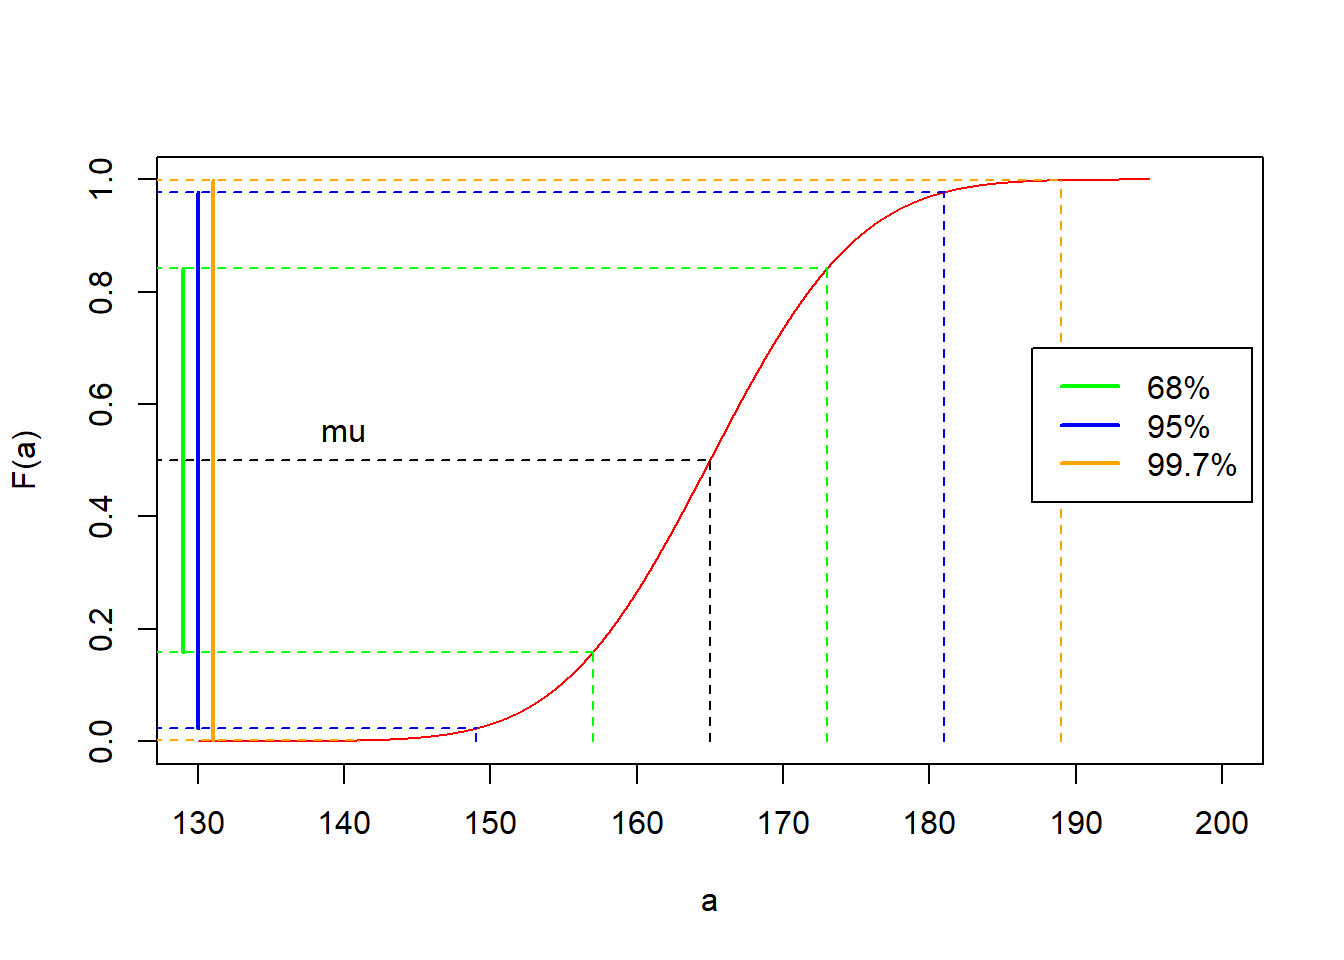
\includegraphics{_main_files/figure-latex/unnamed-chunk-3-1.pdf}

\hypertarget{gruxe1fico-de-sectores-pie}{%
\section{Gráfico de sectores (pie)}\label{gruxe1fico-de-sectores-pie}}

También podemos visualizar las frecuencias relativas con un gráfico de sectores.

El área del círculo representa el 100\% de las observaciones (proporción = 1) y las secciones las frecuencias relativas de cada resultado.

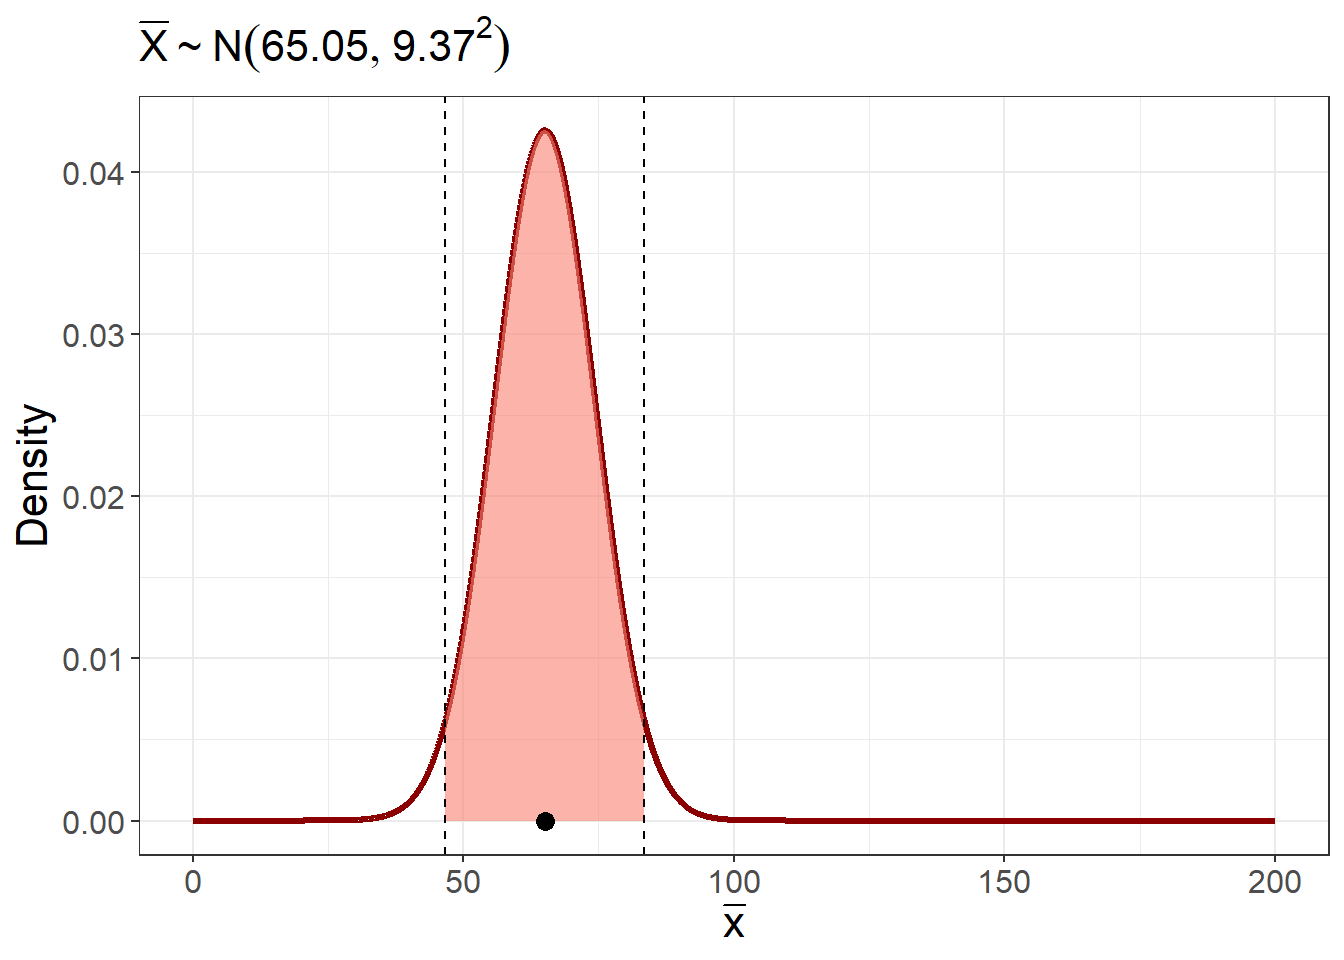
\includegraphics{_main_files/figure-latex/unnamed-chunk-4-1.pdf}

\hypertarget{variables-categuxf3ricas-ordinales}{%
\section{Variables categóricas ordinales}\label{variables-categuxf3ricas-ordinales}}

El tipo de leucocito de los ejemplos anteriores es una variable nominal \textbf{categórica}. Cada observación pertenece a una categoría (cualidad). Las categorías no siempre tienen un orden determindado.

A veces, las variables \textbf{categóricas} se pueden \textbf{ordenar} cuando cumplen una clasificación natural. Esto permite introducir \textbf{frecuencias acumulativas}.

\textbf{Ejemplo (misofonía)}

Este es un estudio clínico en 123 pacientes que fueron examinados por su grado de misofonía. La misofnía es ansiedad/ira descontrolada producida por ciertos sonidos.

Cada paciente fue evaluado con un cuestionario (AMISO) y se clasificaron en 4 grupos diferentes según la gravedad.

Los resultados del estudio son

\begin{verbatim}
##   [1] 4 2 0 3 0 0 2 3 0 3 0 2 2 0 2 0 0 3 3 0 3 3 2 0 0 0 4 2 2 0 2 0 0 0 3 0 2
##  [38] 3 2 2 0 2 3 0 0 2 2 3 3 0 0 4 3 3 2 0 2 0 0 0 2 2 0 0 2 3 0 1 3 2 4 3 2 3
##  [75] 0 2 3 2 4 1 2 0 2 0 2 0 2 2 4 3 0 3 0 0 0 2 2 1 3 0 0 3 2 1 3 0 4 4 2 3 3
## [112] 3 0 3 2 1 2 3 3 4 2 3 2
\end{verbatim}

Cada observación es el resultado de un experimento aleatorio: medición del nivel de misofonía en un paciente. Esta serie de datos se puede resumir en términos de los resultados en la tabla de frecuencia

\begin{verbatim}
##   outcome ni         fi
## 1       0 41 0.33333333
## 2       1  5 0.04065041
## 3       2 37 0.30081301
## 4       3 31 0.25203252
## 5       4  9 0.07317073
\end{verbatim}

\hypertarget{frecuencias-acumuladas-absolutas-y-relativas}{%
\section{Frecuencias acumuladas absolutas y relativas}\label{frecuencias-acumuladas-absolutas-y-relativas}}

La gravedad de la misofonía es \textbf{categórica} \textbf{ordinal} porque sus resultados pueden ordenarse en relación con su grado.

Cuando los resultados se pueden ordenar, es útil preguntar cuántas observaciones se obtuvieron hasta un resultado dado. Llamamos a este número la \textbf{frecuencia acumulada absoluta} hasta el resultado \(i\):
\[N_i=\sum_{k=1..i} n_k\]
También es útil para calcular la \textbf{proporción} de las observaciones que se obtuvo hasta un resultado dado

\[F_i=\sum_{k=1..i} f_k\]

Podemos agregar estas frecuencias en la \textbf{tabla de frecuencias}

\begin{verbatim}
##   outcome ni         fi  Ni        Fi
## 0       0 41 0.33333333  41 0.3333333
## 1       1  5 0.04065041  46 0.3739837
## 2       2 37 0.30081301  83 0.6747967
## 3       3 31 0.25203252 114 0.9268293
## 4       4  9 0.07317073 123 1.0000000
\end{verbatim}

Por lo tanto, el \textbf{67 \%} de los pacientes tenían misofonía hasta la gravedad \textbf{2} y el \textbf{37 \%} de los pacientes tenían una gravedad inferior o igual a \textbf{1}.

\hypertarget{gruxe1fica-de-frecuencia-acumulada}{%
\section{Gráfica de frecuencia acumulada}\label{gruxe1fica-de-frecuencia-acumulada}}

\(F_i\) es una cantidad importante porque nos permite definir la acumulación de probabilidades hasta niveles intermedios.

La probabilidad de un nivel intermedio \(x\) (\(i\leq x< i+1\)) es solo la acumulación hasta el nivel inferior \(F_x=F_i\).

\(F_x\) es por lo tanto una función de rango \textbf{continuo}. Podemos dibujarla con respecto a los resultados.

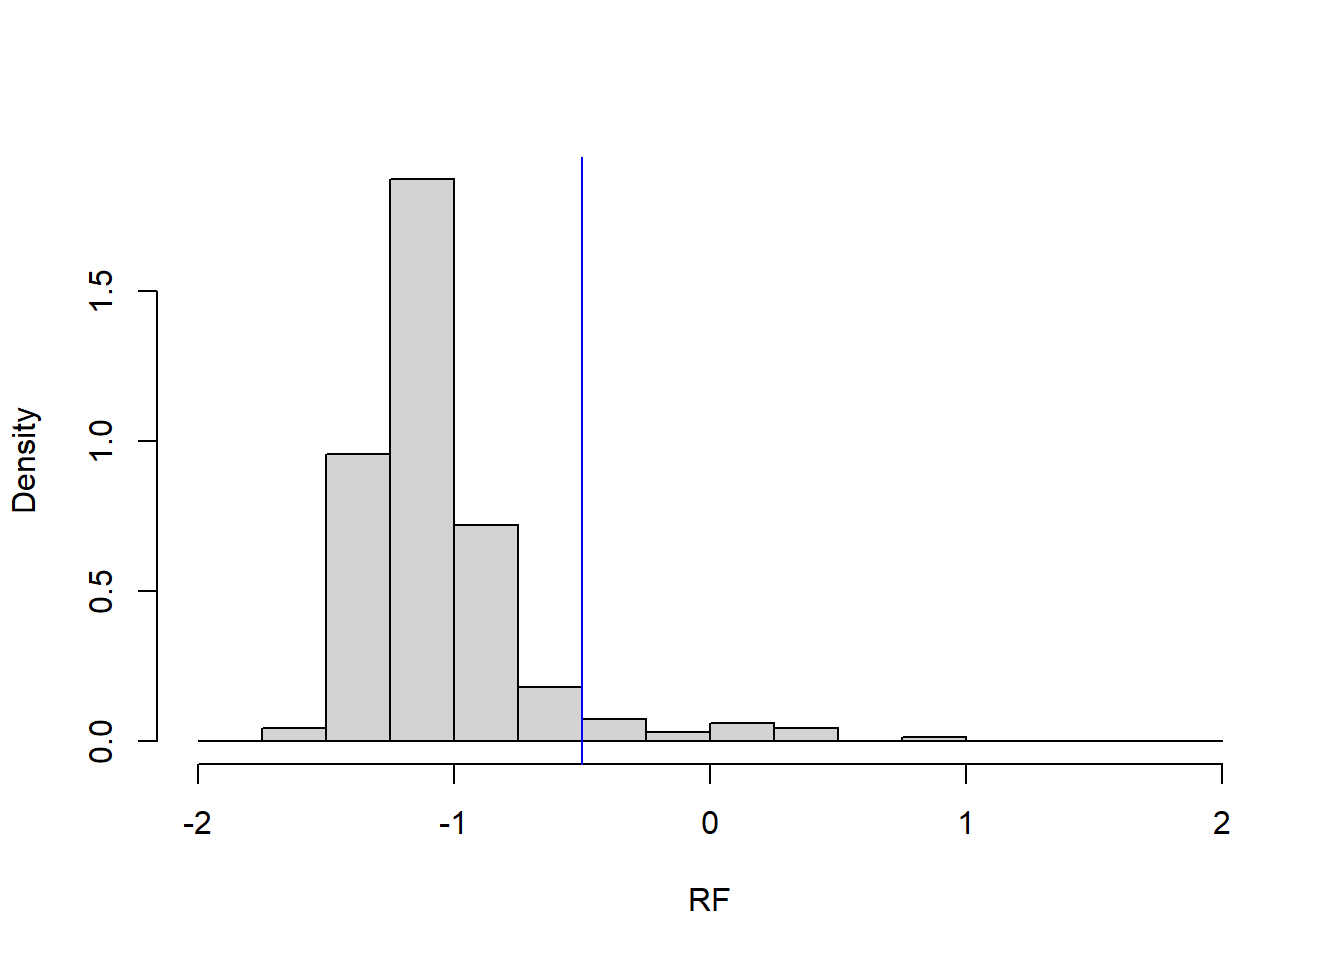
\includegraphics{_main_files/figure-latex/unnamed-chunk-8-1.pdf}

Por lo tanto, podemos decir que el \textbf{67 \%} de los pacientes tenían misofonía hasta gravedad \(2.3\), aunque \(2.3\) no es un resultado observado.

\hypertarget{variables-numuxe9ricas}{%
\section{Variables numéricas}\label{variables-numuxe9ricas}}

El resultado de un experimento aleatorio puede producir un número. Si el número es \textbf{discreto}, podemos generar una tabla de frecuencias, con frecuencias absolutas, relativas y acumulativas, e ilustrarlas con gráficos de barras, de sectores y acumulativos.

Cuando el número es \textbf{continuo} las frecuencias no son útiles, lo más probable es que observemos o no un número contínuo en particular.

\textbf{Ejemplo (misofonía)}

Los investigadores se preguntaron si la convexidad de la mandíbula afectaría la gravedad de la misofonía. La hipótesis científica es que el ángulo de convexidad de la mandíbula puede influir en el oído y su sensibilidad. Estos son los resultados de la convexidad de la mandíbula (grados) para cada paciente:

\begin{verbatim}
##   [1]  7.97 18.23 12.27  7.81  9.81 13.50 19.30  7.70 12.30  7.90 12.60 19.00
##  [13]  7.27 14.00  5.40  8.00 11.20  7.75  7.94 16.69  7.62  7.02  7.00 19.20
##  [25]  7.96 14.70  7.24  7.80  7.90  4.70  4.40 14.00 14.40 16.00  1.40  9.76
##  [37]  7.90  7.90  7.40  6.30  7.76  7.30  7.00 11.23 16.00  7.90  7.29  6.91
##  [49]  7.10 13.40 11.60 -1.00  6.00  7.82  4.80 11.00  9.00 11.50 16.00 15.00
##  [61]  1.40 16.80  7.70 16.14  7.12 -1.00 17.00  9.26 18.70  3.40 21.30  7.50
##  [73]  6.03  7.50 19.00 19.01  8.10  7.80  6.10 15.26  7.95 18.00  4.60 15.00
##  [85]  7.50  8.00 16.80  8.54  7.00 18.30  7.80 16.00 14.00 12.30 11.40  8.50
##  [97]  7.00  7.96 17.60 10.00  3.50  6.70 17.00 20.26  6.64  1.80  7.02  2.46
## [109] 19.00 17.86  6.10  6.64 12.00  6.60  8.70 14.05  7.20 19.70  7.70  6.02
## [121]  2.50 19.00  6.80
\end{verbatim}

\hypertarget{transformando-datos-continuos}{%
\section{Transformando datos continuos}\label{transformando-datos-continuos}}

Como los resultados continuos no se pueden contar (de manera informativa), los transformamos en variables categóricas ordenadas.

\begin{enumerate}
\def\labelenumi{\arabic{enumi})}
\tightlist
\item
  Primero cubrimos el rango de las observaciones en intervalos regulares del mismo tamaño (contenedores)
\end{enumerate}

\begin{verbatim}
## [1] "[-1.02,3.46]" "(3.46,7.92]"  "(7.92,12.4]"  "(12.4,16.8]"  "(16.8,21.3]"
\end{verbatim}

\begin{enumerate}
\def\labelenumi{\arabic{enumi})}
\setcounter{enumi}{1}
\tightlist
\item
  Luego mapeamos cada observación a su intervalo: creando una variable categórica \textbf{ordenada}; en este caso con 5 resultados posibles
\end{enumerate}

\begin{verbatim}
##   [1] "(7.92,12.4]"  "(16.8,21.3]"  "(7.92,12.4]"  "(3.46,7.92]"  "(7.92,12.4]" 
##   [6] "(12.4,16.8]"  "(16.8,21.3]"  "(3.46,7.92]"  "(7.92,12.4]"  "(3.46,7.92]" 
##  [11] "(12.4,16.8]"  "(16.8,21.3]"  "(3.46,7.92]"  "(12.4,16.8]"  "(3.46,7.92]" 
##  [16] "(7.92,12.4]"  "(7.92,12.4]"  "(3.46,7.92]"  "(7.92,12.4]"  "(12.4,16.8]" 
##  [21] "(3.46,7.92]"  "(3.46,7.92]"  "(3.46,7.92]"  "(16.8,21.3]"  "(7.92,12.4]" 
##  [26] "(12.4,16.8]"  "(3.46,7.92]"  "(3.46,7.92]"  "(3.46,7.92]"  "(3.46,7.92]" 
##  [31] "(3.46,7.92]"  "(12.4,16.8]"  "(12.4,16.8]"  "(12.4,16.8]"  "[-1.02,3.46]"
##  [36] "(7.92,12.4]"  "(3.46,7.92]"  "(3.46,7.92]"  "(3.46,7.92]"  "(3.46,7.92]" 
##  [41] "(3.46,7.92]"  "(3.46,7.92]"  "(3.46,7.92]"  "(7.92,12.4]"  "(12.4,16.8]" 
##  [46] "(3.46,7.92]"  "(3.46,7.92]"  "(3.46,7.92]"  "(3.46,7.92]"  "(12.4,16.8]" 
##  [51] "(7.92,12.4]"  "[-1.02,3.46]" "(3.46,7.92]"  "(3.46,7.92]"  "(3.46,7.92]" 
##  [56] "(7.92,12.4]"  "(7.92,12.4]"  "(7.92,12.4]"  "(12.4,16.8]"  "(12.4,16.8]" 
##  [61] "[-1.02,3.46]" "(12.4,16.8]"  "(3.46,7.92]"  "(12.4,16.8]"  "(3.46,7.92]" 
##  [66] "[-1.02,3.46]" "(16.8,21.3]"  "(7.92,12.4]"  "(16.8,21.3]"  "[-1.02,3.46]"
##  [71] "(16.8,21.3]"  "(3.46,7.92]"  "(3.46,7.92]"  "(3.46,7.92]"  "(16.8,21.3]" 
##  [76] "(16.8,21.3]"  "(7.92,12.4]"  "(3.46,7.92]"  "(3.46,7.92]"  "(12.4,16.8]" 
##  [81] "(7.92,12.4]"  "(16.8,21.3]"  "(3.46,7.92]"  "(12.4,16.8]"  "(3.46,7.92]" 
##  [86] "(7.92,12.4]"  "(12.4,16.8]"  "(7.92,12.4]"  "(3.46,7.92]"  "(16.8,21.3]" 
##  [91] "(3.46,7.92]"  "(12.4,16.8]"  "(12.4,16.8]"  "(7.92,12.4]"  "(7.92,12.4]" 
##  [96] "(7.92,12.4]"  "(3.46,7.92]"  "(7.92,12.4]"  "(16.8,21.3]"  "(7.92,12.4]" 
## [101] "(3.46,7.92]"  "(3.46,7.92]"  "(16.8,21.3]"  "(16.8,21.3]"  "(3.46,7.92]" 
## [106] "[-1.02,3.46]" "(3.46,7.92]"  "[-1.02,3.46]" "(16.8,21.3]"  "(16.8,21.3]" 
## [111] "(3.46,7.92]"  "(3.46,7.92]"  "(7.92,12.4]"  "(3.46,7.92]"  "(7.92,12.4]" 
## [116] "(12.4,16.8]"  "(3.46,7.92]"  "(16.8,21.3]"  "(3.46,7.92]"  "(3.46,7.92]" 
## [121] "[-1.02,3.46]" "(16.8,21.3]"  "(3.46,7.92]"
\end{verbatim}

Por tanto, en lugar de decir que el primer paciente tenía un ángulo de convexidad de \(7.97\), decimos que su ángulo estaba entre el intervalo (o \textbf{bin}) \((7.92,12.4]\).

Ningún otro paciente tenía un ángulo de \(7.97\), pero muchos tenían ángulos entre \((7.92,12.4]\).

\hypertarget{tabla-de-frecuencias-para-una-variable-continua}{%
\section{Tabla de frecuencias para una variable continua}\label{tabla-de-frecuencias-para-una-variable-continua}}

Para una partición regular dada del intervalo de resultados en intervalos, podemos producir una tabla de frecuencias como antes

\begin{verbatim}
##        outcome ni         fi  Ni         Fi
## 1 [-1.02,3.46]  8 0.06504065   8 0.06504065
## 2  (3.46,7.92] 51 0.41463415  59 0.47967480
## 3  (7.92,12.4] 26 0.21138211  85 0.69105691
## 4  (12.4,16.8] 20 0.16260163 105 0.85365854
## 5  (16.8,21.3] 18 0.14634146 123 1.00000000
\end{verbatim}

\hypertarget{histograma}{%
\section{Histograma}\label{histograma}}

El histograma es la gráfica de \(n_i\) o \(f_i\) Vs los resultados en intervalos (bins). El histograma depende del tamaño de los bins.

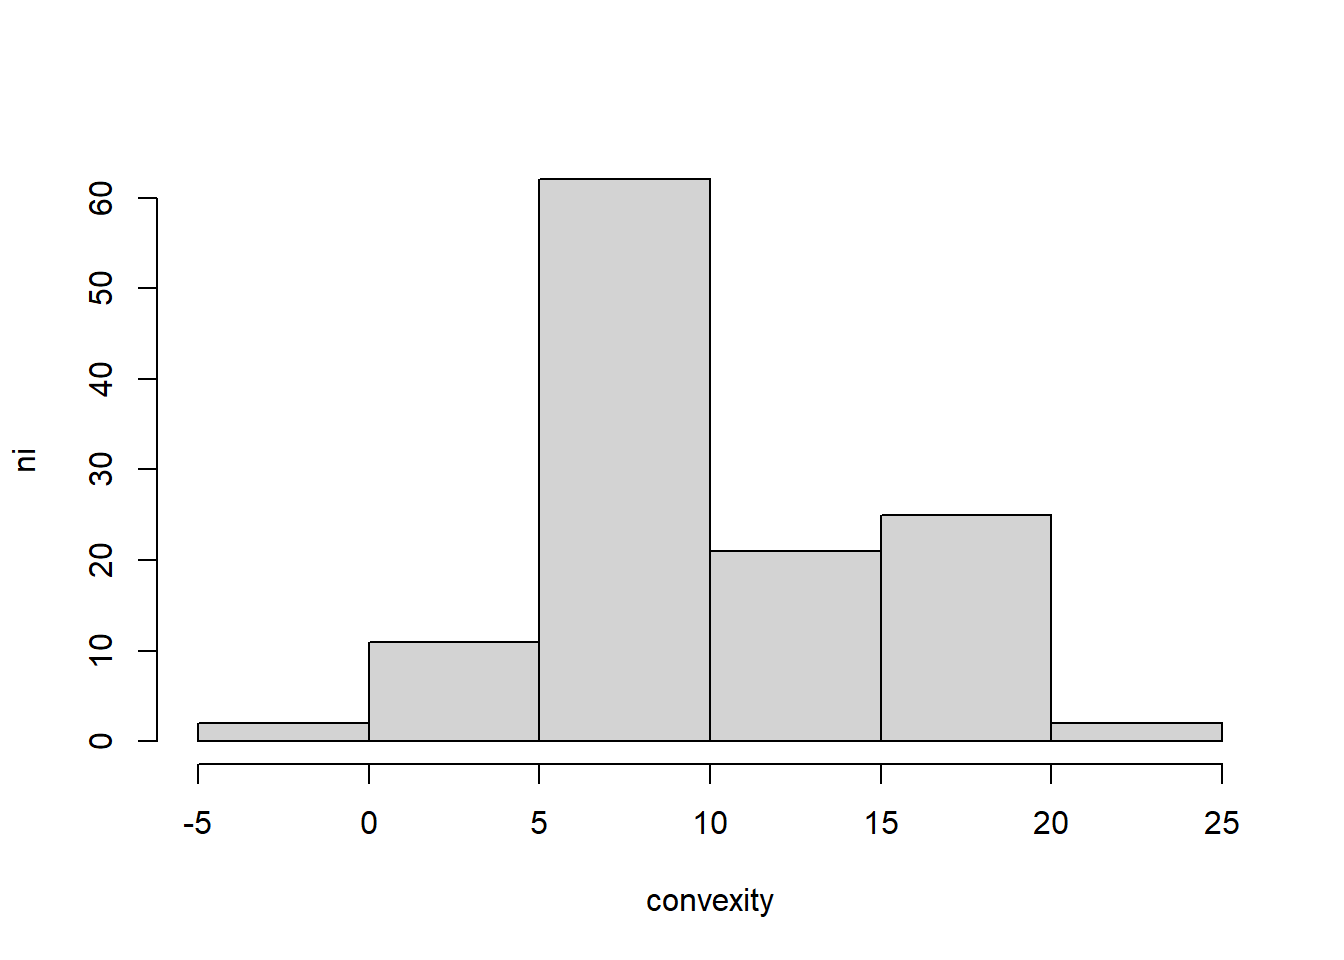
\includegraphics{_main_files/figure-latex/unnamed-chunk-13-1.pdf}

Este es un histograma con 20 bins.

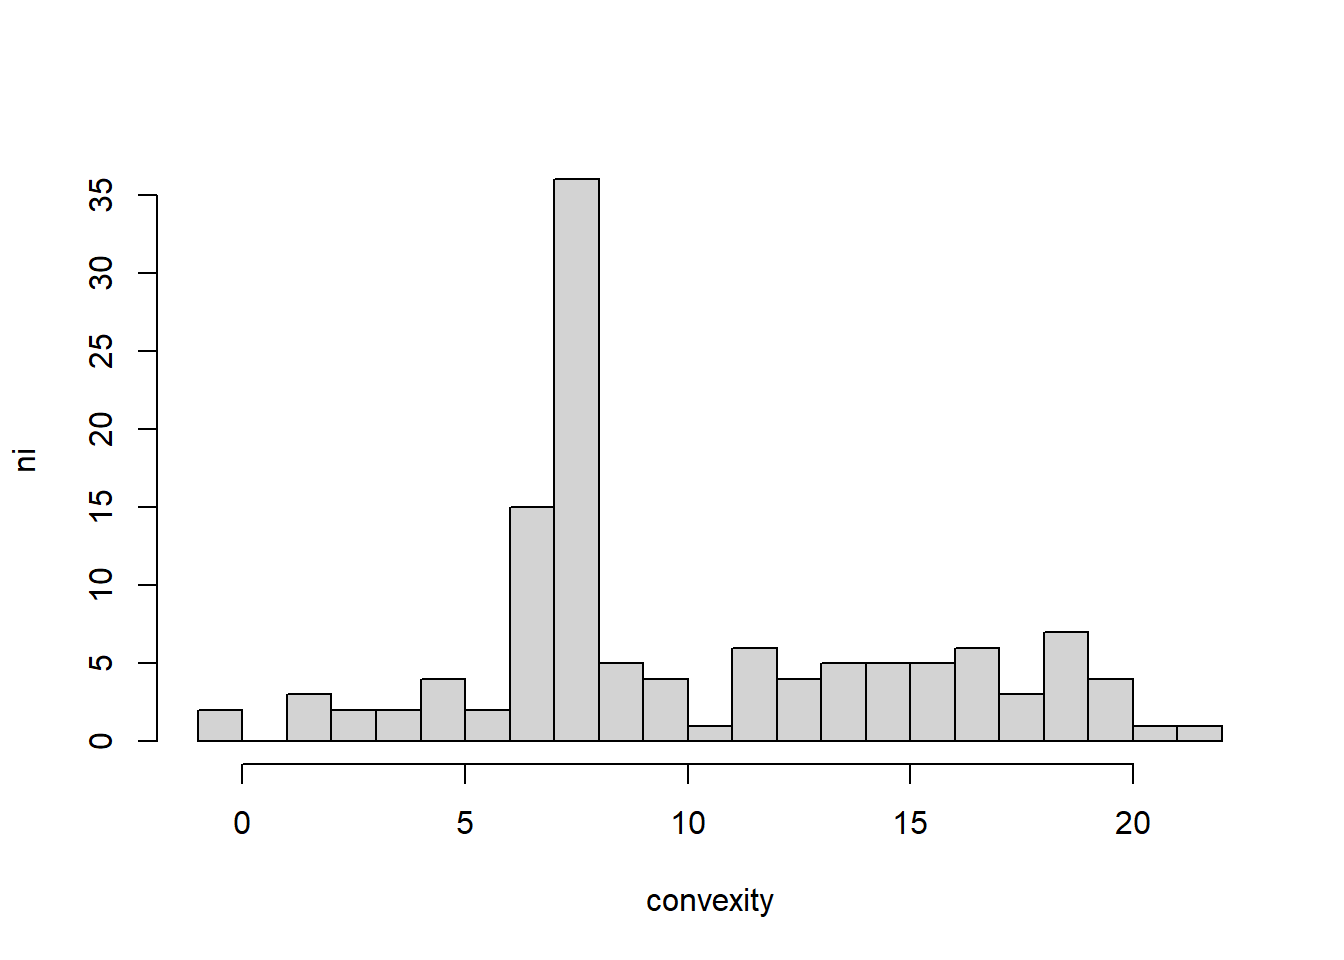
\includegraphics{_main_files/figure-latex/unnamed-chunk-14-1.pdf}

Vemos que la mayoría de las personas tienen ángulos dentro de \((7, 8]\)

\hypertarget{gruxe1fica-de-frecuencia-acumulada-1}{%
\section{Gráfica de frecuencia acumulada}\label{gruxe1fica-de-frecuencia-acumulada-1}}

También podemos graficar \(F_x\) contra los resultados. Como \(F_x\) es de rango continuo, podemos ordenar las observaciones (\(x_1 <... x_j < x_{j+1} < x_n\)) y por lo tanto

\[F_x = \frac{k}{n}\]

para \(x_{k} \leq x < x_{k+1}\).

\(F_x\) se conoce como la \textbf{distribución} de los datos. \(F_x\) no depende del tamaño del bin. Sin embargo, su \textbf{resolución} depende de la cantidad de datos.

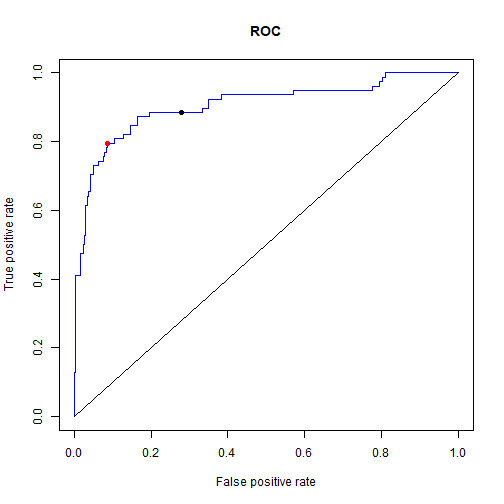
\includegraphics{_main_files/figure-latex/unnamed-chunk-15-1.pdf}

\hypertarget{estaduxedsticas-de-resumen}{%
\section{Estadísticas de resumen}\label{estaduxedsticas-de-resumen}}

Las estadísticas de resumen son números calculados a partir de los datos que nos dicen características importantes de las variables numéricas (discretas o continuas).

Por ejemplo, tenemos estadísticas que describen los valores extremos:

\begin{itemize}
\tightlist
\item
  \textbf{mínimo}: el resultado mínimo observado
\item
  \textbf{máximo}: el resultado máximo observado
\end{itemize}

\hypertarget{promedio-media-muestral}{%
\section{Promedio (media muestral)}\label{promedio-media-muestral}}

Una estadística importante que describe el valor central de los resultados (dónde esperar la mayoría de las observaciones) es el \textbf{promedio}

\[\bar{x}=\frac{1}{N} \sum_{j=1..N} x_j\]

donde \(x_j\) es la \textbf{observación} \(j\) de un total de \(N\).

\textbf{Ejemplo (Misofonía)}

La convexidad promedio se puede calcular directamente a partir de las \textbf{observaciones}

\(\bar{x}= \frac{1}{N}\sum_j x_j\)

\(= \frac{1}{N}(7.97 + 18.23 + 12.27... + 6.80) = 10.19894\)

Para variables \textbf{categóricamente ordenadas}, podemos usar las frecuencias relativas para calcular el promedio

\(\bar{x}=\frac{1}{N}\sum_{i=1...N} x_j=\frac{1}{N}\sum_{i=1...M} x_i*n_ {i}\)
\[=\sum_{i=1...M} x_i*f_{i}\]

donde pasamos de sumar \(N\) \textbf{observaciones} a sumar \(M\) \textbf{resultados}.

La forma \(\bar{x}= \sum_{i = 1...M} x_i f_i\) muestra que el promedio es el \textbf{centro de gravedad} de los resultados. Como si cada resultado tuviera una densidad de masa dada por \(f_i\).

\textbf{Ejemplo (Misofonía)}

La \textbf{severidad} promedio de la misofonía en el estudio se puede calcular a partir de las frecuencias relativas de los \textbf{resultados}

\begin{verbatim}
##   outcome ni         fi
## 1       0 41 0.33333333
## 2       1  5 0.04065041
## 3       2 37 0.30081301
## 4       3 31 0.25203252
## 5       4  9 0.07317073
\end{verbatim}

\(\bar{x}=0*f_{0}+1*f_{1}+2*f_{2}+3*f_{3}+4*f_{4}=1.691057\)

\hypertarget{promedio}{%
\section{Promedio}\label{promedio}}

El promedio es también el centro de gravedad de las variables continuas. Ese es el punto donde las frecuencias reativas se equilibran.

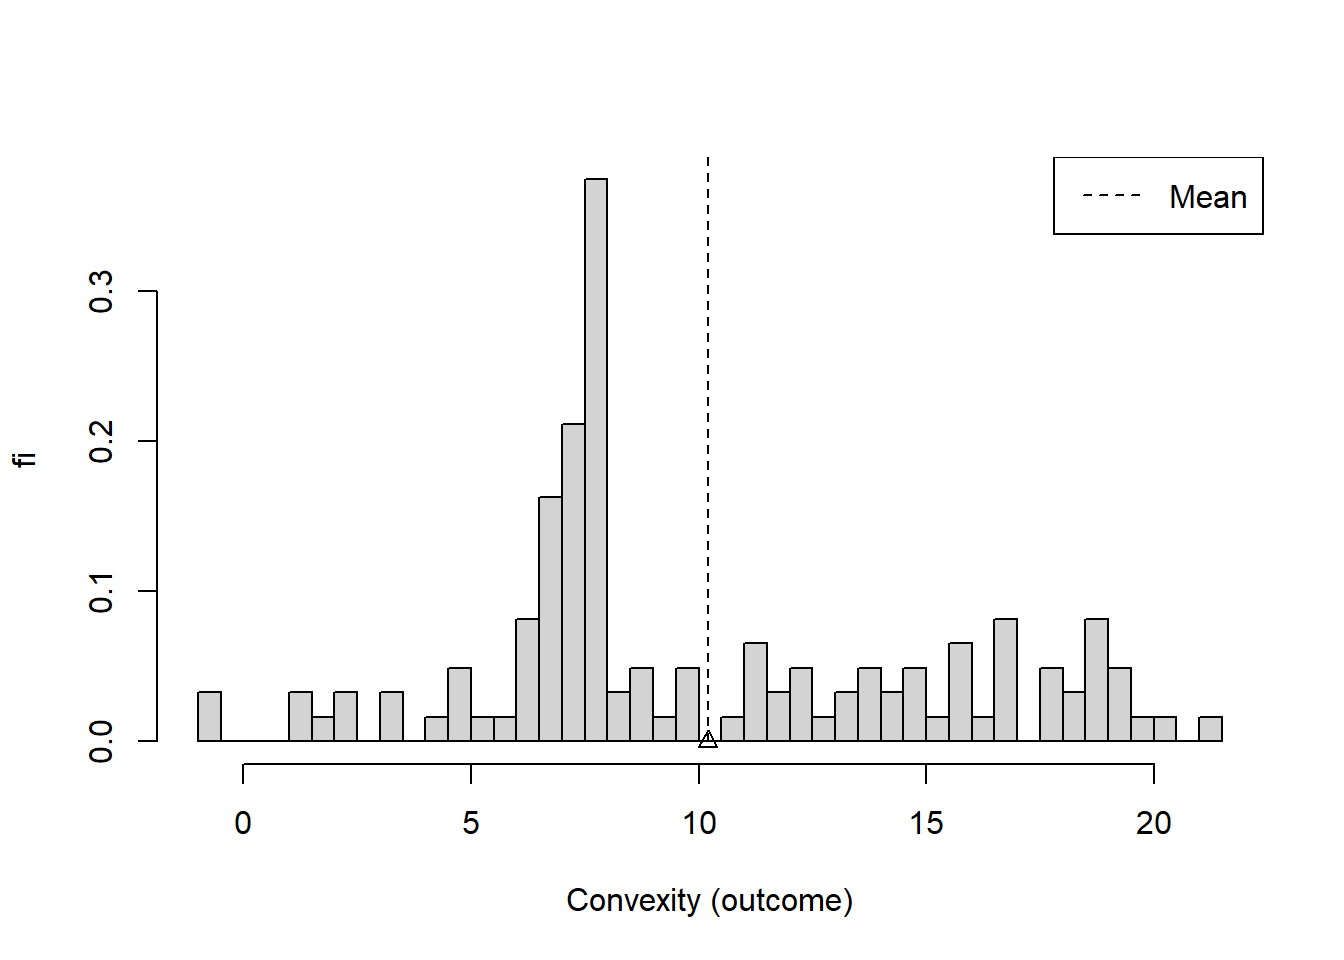
\includegraphics{_main_files/figure-latex/unnamed-chunk-17-1.pdf}

\hypertarget{mediana}{%
\section{mediana}\label{mediana}}

Otra medida de centralidad es la mediana. La mediana \(x_m\), o \(q_{0.5}\), es el valor por debajo del cual encontramos la mitad de las observaciones. Cuando ordenamos las observaciones \(x_1 <... x_j < x_{j+1} < x_N\), las contamos hasta encontrar la mitad de ellas. \(x_m\) es tal que

\[\sum_{i\leq m} 1 = \frac{N}{2}\]
\textbf{Ejemplo (Misofonía)}

Si ordenamos los ángulos de convexidad, vemos que \(62\) observaciones (individuos) (\(N/2 \sim 123/2\)) están por debajo de \(7.96\). La \textbf{convexidad mediana} es por lo tanto \(q_{0.5}=x_{62}=7.96\)

\begin{verbatim}
##  [1] -1.00 -1.00  1.40  1.40  1.80  2.46  2.50  3.40  3.50  4.40  4.60  4.70
## [13]  4.80  5.40  6.00  6.02  6.03  6.10  6.10  6.30  6.60  6.64  6.64  6.70
## [25]  6.80  6.91  7.00  7.00  7.00  7.00  7.02  7.02  7.10  7.12  7.20  7.24
## [37]  7.27  7.29  7.30  7.40  7.50  7.50  7.50  7.62  7.70  7.70  7.70  7.75
## [49]  7.76  7.80  7.80  7.80  7.81  7.82  7.90  7.90  7.90  7.90  7.90  7.94
## [61]  7.95  7.96
\end{verbatim}

\begin{verbatim}
##  [1]  7.96  7.97  8.00  8.00  8.10  8.50  8.54  8.70  9.00  9.26  9.76  9.81
## [13] 10.00 11.00 11.20 11.23 11.40 11.50 11.60 12.00 12.27 12.30 12.30 12.60
## [25] 13.40 13.50 14.00 14.00 14.00 14.05 14.40 14.70 15.00 15.00 15.26 16.00
## [37] 16.00 16.00 16.00 16.14 16.69 16.80 16.80 17.00 17.00 17.60 17.86 18.00
## [49] 18.23 18.30 18.70 19.00 19.00 19.00 19.00 19.01 19.20 19.30 19.70 20.26
## [61] 21.30
\end{verbatim}

\begin{verbatim}
## [1] 7.96
\end{verbatim}

En términos de frecuencias, \(q_{0.5}\) hace que la frecuencia acumulada \(F_x\) sea igual a \(0.5\)

\[\sum_{i = 0, ... m} f_i =F_{q_{0.5}}=0.5\]
o

\[q_{0.5}=F^{-1}(0.5)\]

En el gráfico de distribución, la mediana es el valor de \(x\) en el que se encuentra la mitad del máximo de \(F\).

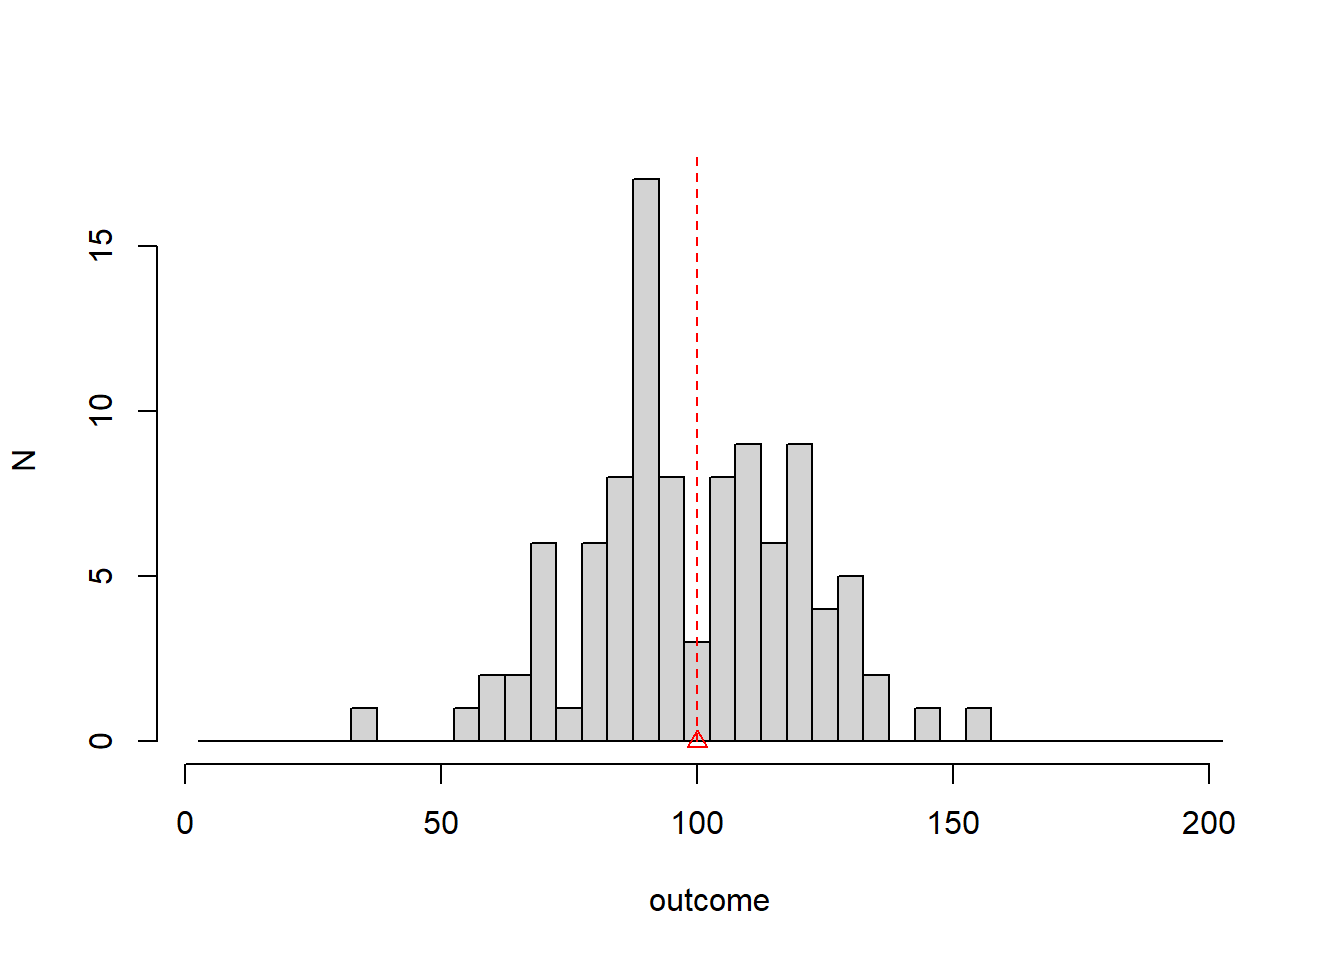
\includegraphics{_main_files/figure-latex/unnamed-chunk-20-1.pdf}

El promedio y la mediana no siempre son iguales.

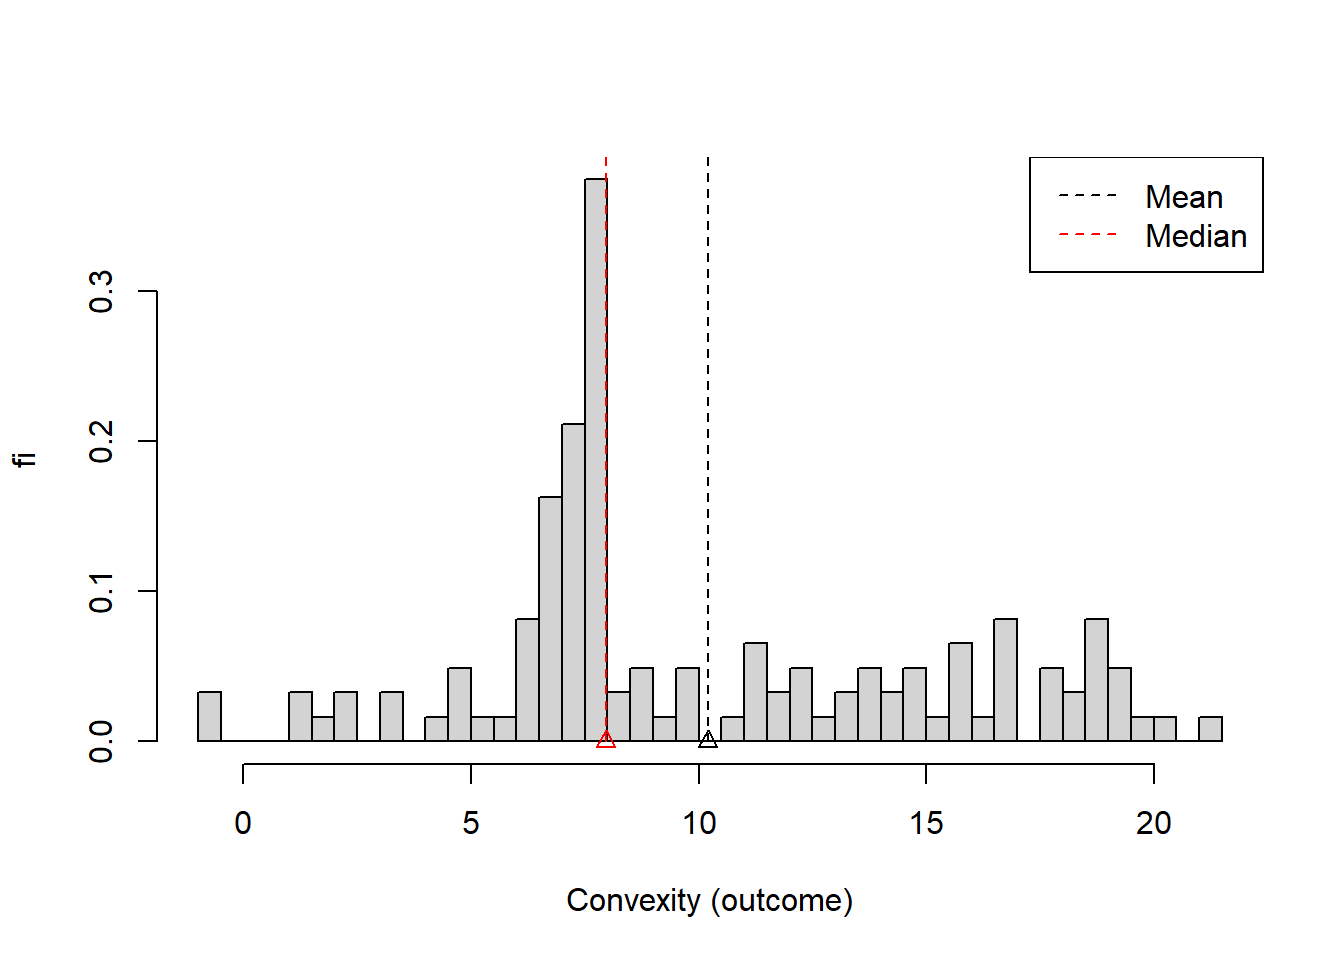
\includegraphics{_main_files/figure-latex/unnamed-chunk-21-1.pdf}

\hypertarget{dispersiuxf3n}{%
\section{Dispersión}\label{dispersiuxf3n}}

Otras estadísticas de resumen importantes de las observaciones son las de \textbf{dispersión}.

Muchos experimentos pueden compartir su media, pero difieren en cuán \textbf{dispersos} son los valores.

La dispersión de las observaciones es una medida del \textbf{ruido}.

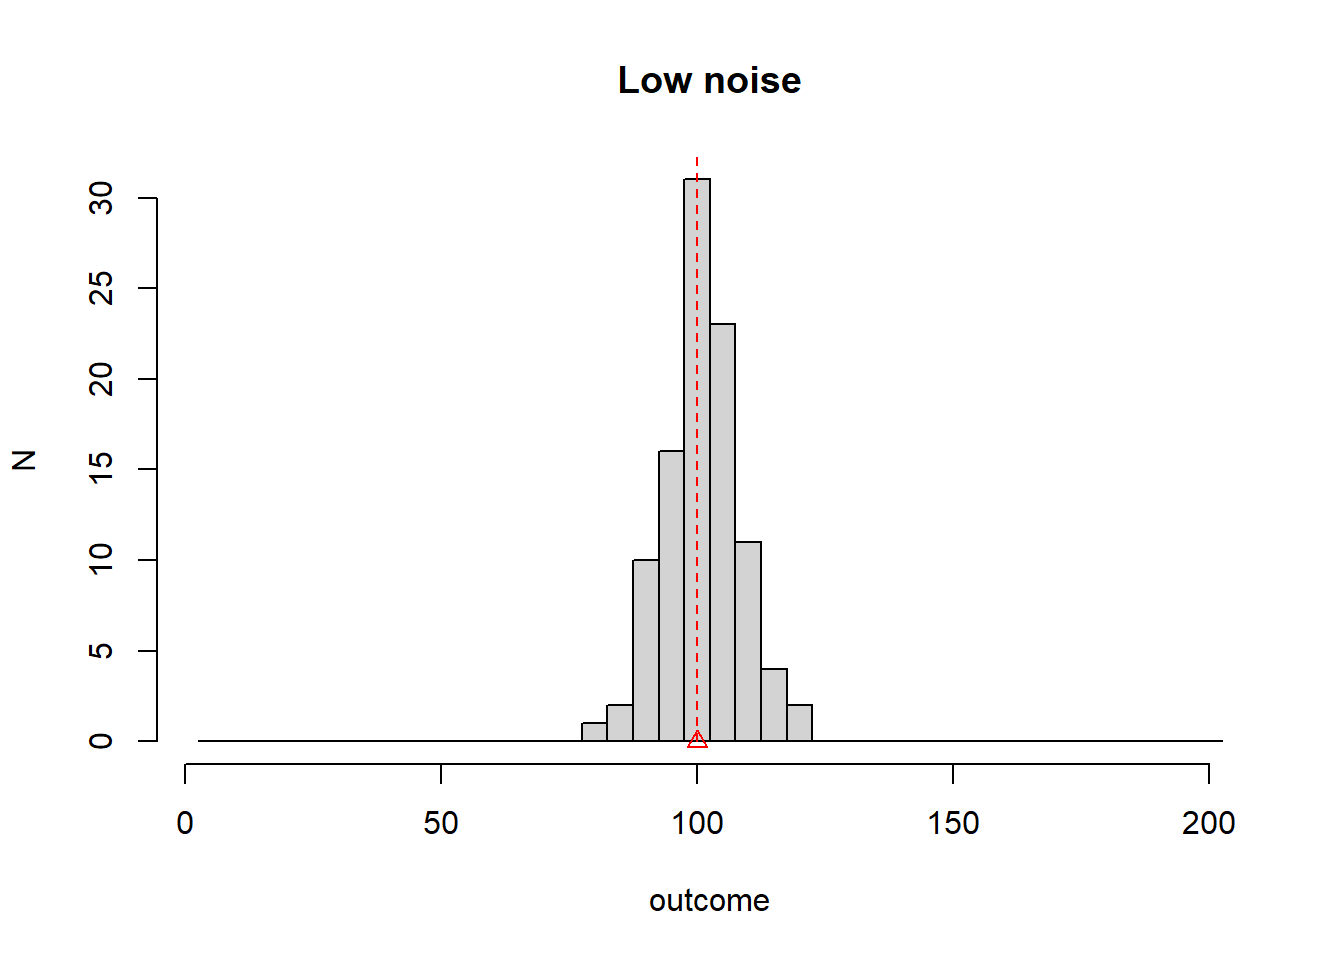
\includegraphics{_main_files/figure-latex/unnamed-chunk-22-1.pdf} 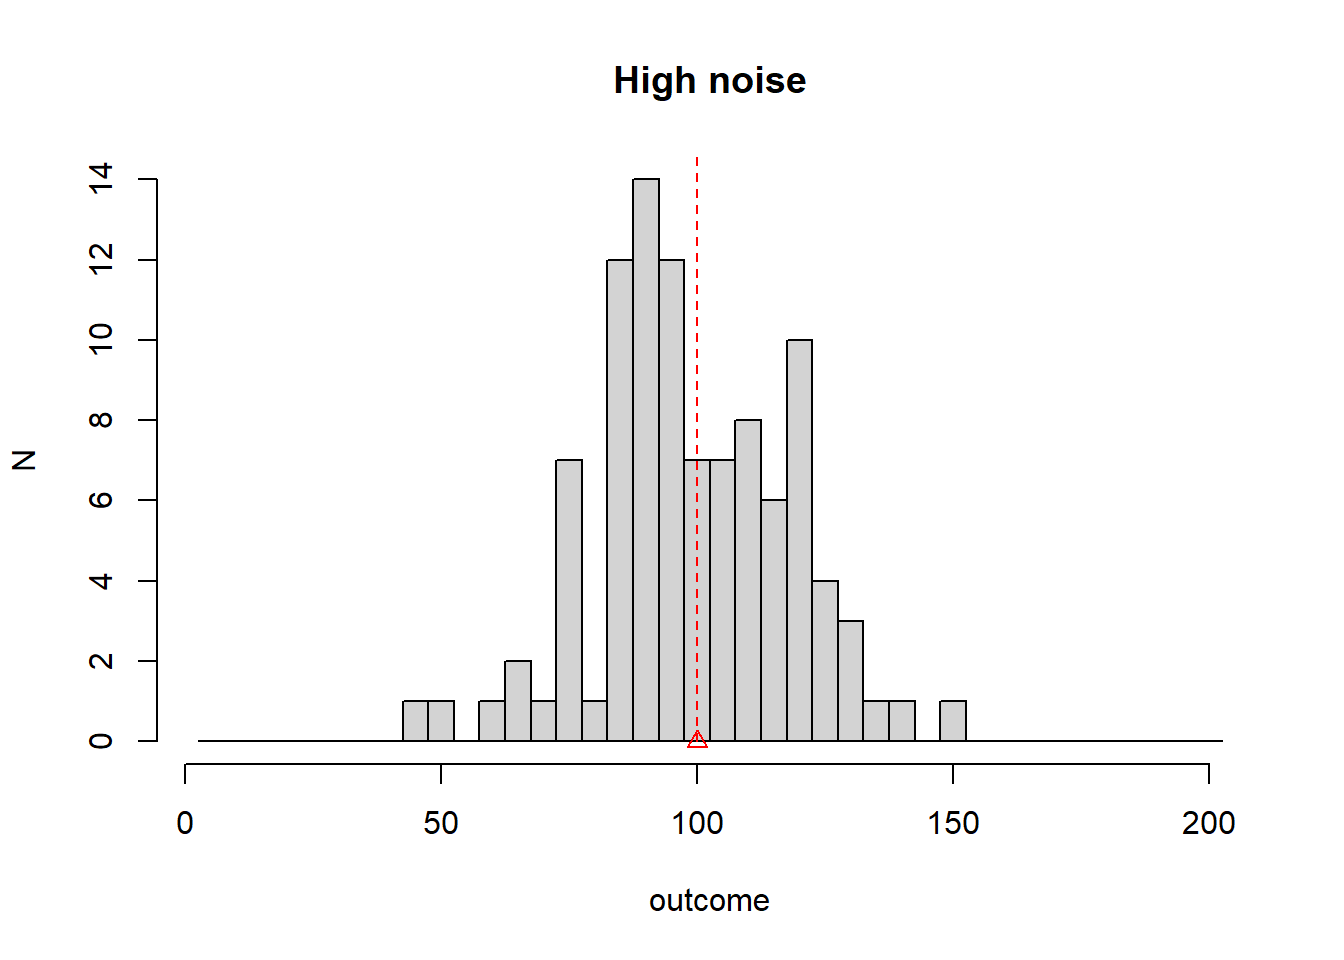
\includegraphics{_main_files/figure-latex/unnamed-chunk-22-2.pdf}

\hypertarget{variaciuxf3n-de-la-muestra}{%
\section{Variación de la muestra}\label{variaciuxf3n-de-la-muestra}}

La dispersión sobre la media se mide con la varianza muestral

\[s^2=\frac{1}{N-1} \sum_{j=1..N} (x_j-\bar{x})^2\]

Este número, mide la distancia cuadrada promedio de las \textbf{observaciones} al promedio. La razón de \(N-1\) se explicará cuando hablemos de inferencia, cuando estudiemos la dispersión de \(\bar{x}\), además de la dispersión de las observaciones.

En términos de las frecuencias de las variables \textbf{categóricas y ordenadas}

\[s^2=\frac{N}{N-1} \sum_{i=1... M} (x_i-\bar{x})^2 f_i\]

\(s^2\) se puede considerar como el \textbf{momento de inercia} de las observaciones.

La raíz cuadrada de la varianza de la muestra se denomina \textbf{desviación estándar} \(s\).

\textbf{Ejemplo (Misofonía)}

La desviación estándar del ángulo de convexidad es

\(s= [\frac{1}{123-1}((7.97-10.19894)^2+ (18.23-10.19894)^2\)
\(+ (12.27-10.19894)^2 + ...)]^{1/2} = 5.086707\)

La convexidad de la mandíbula se desvía de su media en \(5.086707\).

\hypertarget{rango-intercuartuxedlico-iqr}{%
\section{Rango intercuartílico (IQR)}\label{rango-intercuartuxedlico-iqr}}

La dispersión de los datos también se puede medir con respecto a la mediana usando el \textbf{rango intercuartílico}:

\begin{enumerate}
\def\labelenumi{\arabic{enumi})}
\tightlist
\item
  Definimos el \textbf{primer} cuartil como el valor \(x_m\) que hace que la frecuencia acumulada \(F_{q_{0.25}}\) sea igual a \(0.25\) (\(x\) donde hemos acumulado una cuarta parte de las observaciones)
\end{enumerate}

\[F_{q_{0.25}}=0.25\]

\begin{enumerate}
\def\labelenumi{\arabic{enumi})}
\tightlist
\item
  Definimos el \textbf{tercer} cuartil como el valor \(x_m\) que hace que la frecuencia acumulada \(F_{q_{0.75}}\) sea igual a \(0.75\) (\(x\) donde hemos acumulado tres cuartos de observaciones)
\end{enumerate}

\[F_{q_{0.75}}=0.75\]

\begin{enumerate}
\def\labelenumi{\arabic{enumi})}
\setcounter{enumi}{2}
\tightlist
\item
  El \textbf{rango intercuartílico} (IQR) es \(IQR=q_{0.75} - q_{0.25}\). Esa es la distancia entre el tercer y el primer cuartil y captura el \(50\%\) central de las observaciones
\end{enumerate}

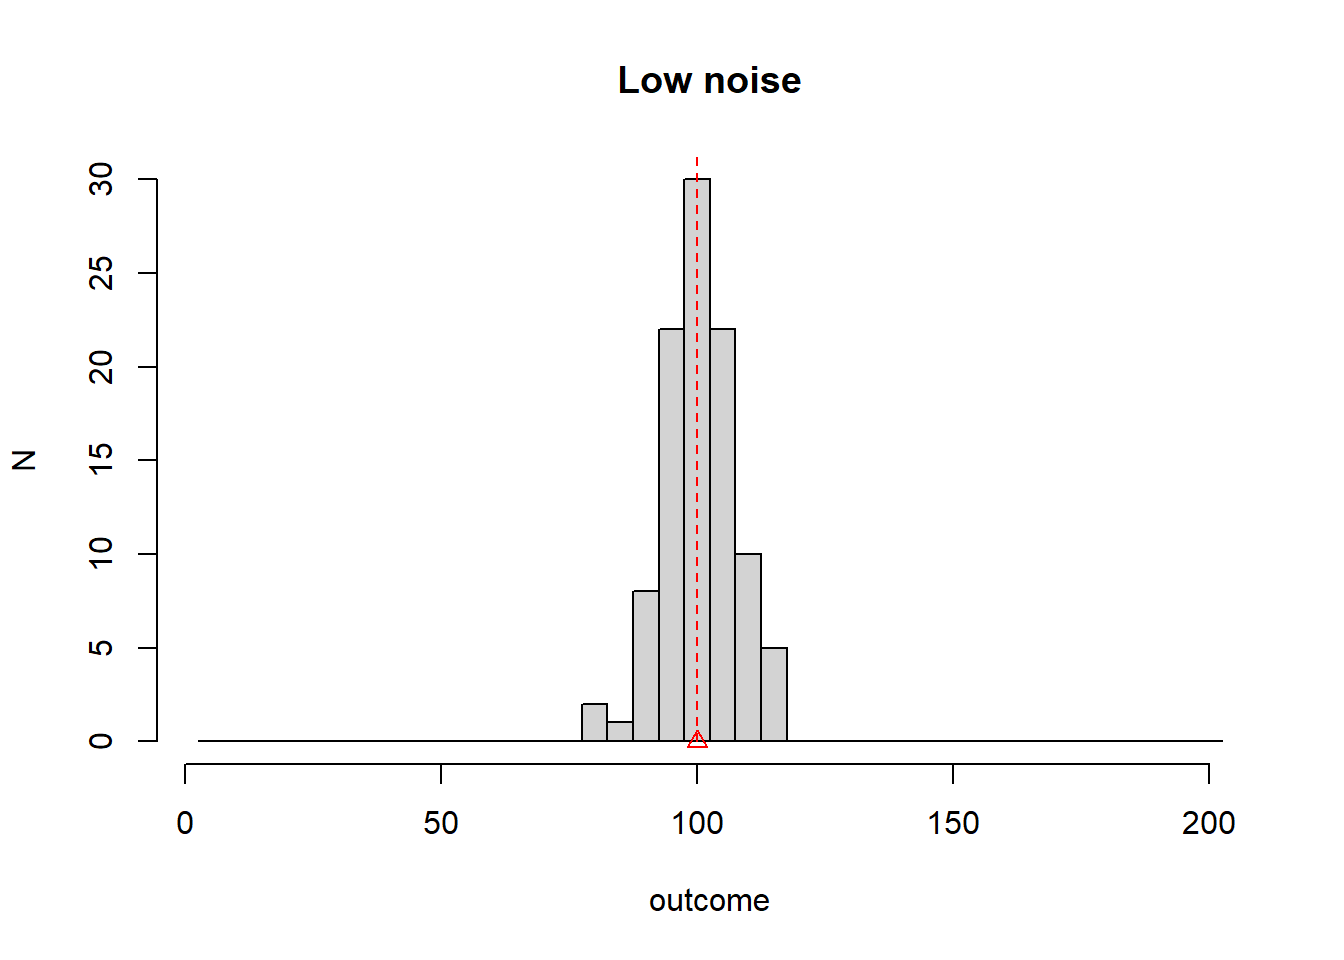
\includegraphics{_main_files/figure-latex/unnamed-chunk-23-1.pdf}

\hypertarget{diagrama-de-caja}{%
\section{Diagrama de caja}\label{diagrama-de-caja}}

El rango intercuartílico, la mediana y los \(5\%\) y \(95\%\) de los datos se pueden visualizar en un \textbf{diagrama de caja}.

En el diagrama de caja, los valores de los resultados están en el eje y. El IQR es la caja, la mediana es la línea del medio y los bigotes marcan los \(5\%\) y \(95\%\) de los datos.

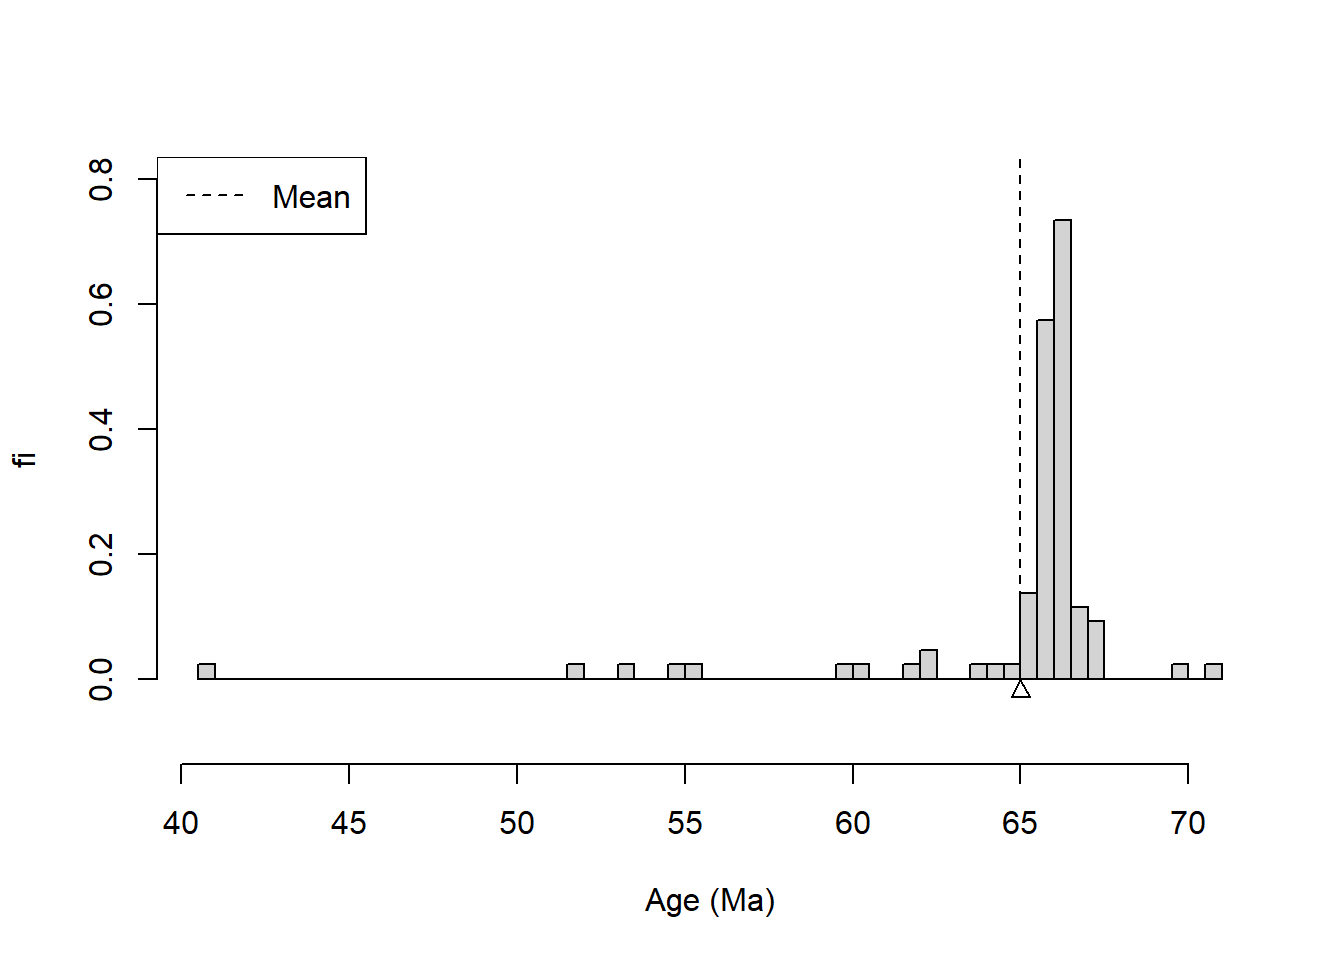
\includegraphics{_main_files/figure-latex/unnamed-chunk-24-1.pdf}

\hypertarget{preguntas}{%
\section{Preguntas}\label{preguntas}}

\textbf{1)} En el siguiente diagrama de caja, el primer cuartil y el segundo cuartil de los datos son:

\textbf{\(\qquad\)a:} \((-1.00, 21.30)\); \textbf{\(\qquad\)b:} \((-1.00, 7.02)\); \textbf{\(\qquad\)c:} \((7.02, 7.96)\); \textbf{\(\qquad\)d:} \((7.02, 14.22)\)

\textbf{2)} La principal desventaja de un histograma es que:

\textbf{\(\qquad\)a:} Depende del tamaño del bin; \textbf{\(\qquad\)b:} No se puede utilizar para variables categóricas;
\textbf{\(\qquad\)c:} No se puede usar cuando el tamaño del bin es pequeño;
\textbf{\(\qquad\)d:} Se usa solo para frecuencias relativas;

\textbf{3)} Si las frecuencias acumuladas relativas de un experimento aleatorio con resultados \(\{1,2,3,4\}\) son: \(F(1)=0.15, \qquad F(2)=0.60, \qquad F(3)=0.85, \qquad F(4)=1\).

Entonces la frecuencia relativa para el resultado \(3\) es

\textbf{\(\qquad\)a:} \(0.15\); \textbf{\(\qquad\)b:} \(0.85\); \textbf{\(\qquad\)c:} \(0.45\); \textbf{\(\qquad\)d:} \(0.25\)

\textbf{4)} En una muestra de tamaño \(10\) de un experimento aleatorio obtuvimos los siguientes datos:

\(8,\qquad 3,\qquad 3,\qquad 7,\qquad 3,\qquad 6,\qquad 5,\qquad 10,\qquad 3,\qquad 8\).

El primer cuartil de los datos es:

\textbf{\(\qquad\)a:} \(3.5\); \textbf{\(\qquad\)b:} \(4\); \textbf{\(\qquad\)c:} \(5\); \textbf{\(\qquad\)d:} \(3\)

\textbf{5)} Imaginemos que recopilamos datos para dos cantidades que no son mutuamente excluyentes, por ejemplo, el sexo y la nacionalidad de los pasajeros de un vuelo. Si queremos hacer un solo gráfico circular para los datos, ¿cuál de estas afirmaciones es verdadera?

\textbf{\(\qquad\)a:} Solo podemos hacer un gráfico circular de nacionalidad porque tiene más de dos resultados posibles; \textbf{\(\qquad\)b:} Podemos hacer un gráfico circular para una variable nueva que marca el sexo \textbf{y} la nacionalidad; \textbf{\(\qquad\)c:} Podemos hacer un gráfico circular para la variale sexo o la variable nacionalidad; \textbf{\(\qquad\)d:} Solo podemos elegir si hacemos un gráfico circular para el sexo o un gráfico circular para la nacionalidad.

\hypertarget{ejercicios}{%
\section{Ejercicios}\label{ejercicios}}

\hypertarget{ejercicio-1}{%
\subsubsection{Ejercicio 1}\label{ejercicio-1}}

Hemos realizado un experimento 8 veces con los siguientes resultados

\begin{verbatim}
## [1]  3  3 10  2  6 11  5  4
\end{verbatim}

Responde las siguientes cuestiones:

\begin{itemize}
\tightlist
\item
  Calcula las frecuencias relativas de cada resultado.
\item
  Calcula las frecuencias acumuladas de cada resultado.
\item
  ¿Cuál es el promedio de las observaciones?
\item
  ¿Cuál es la mediana?
\item
  ¿Cuál es el tercer cuartil?
\item
  ¿Cuál es el primer cuartil?
\end{itemize}

\hypertarget{ejercicio-2}{%
\subsubsection{Ejercicio 2}\label{ejercicio-2}}

Hemos realizado un experimento 10 veces con los siguientes resultados

\begin{verbatim}
##  [1] 2.875775 7.883051 4.089769 8.830174 9.404673 0.455565 5.281055 8.924190
##  [9] 5.514350 4.566147
\end{verbatim}

Considera 10 bins de tamaño 1: {[}0,1{]}, (1,2{]}\ldots(9,10).

Responde las siguientes cuestiones:

\begin{itemize}
\item
  Calcula las frecuencias relativas de cada resultado y dibuja el histograma
\item
  Calcula las frecuencias acumulativas de cada resultado y dibuja la gráfica acumulativa.
\item
  Dibuja un diagrama de caja .
\end{itemize}

\hypertarget{probabilidad}{%
\chapter{Probabilidad}\label{probabilidad}}

En este capítulo introduciremos el concepto de probabilidad a partir de frecuencias relativas.

Definiremos los eventos como los elementos sobre los que se aplica la probabilidad. Los eventos compuestos se definirán usando álgebra de conjuntos.

Luego discutiremos el concepto de probabilidad condicional derivado de la probabilidad conjunta de dos eventos.

\hypertarget{experimentos-aleatorios-1}{%
\section{Experimentos aleatorios}\label{experimentos-aleatorios-1}}

Recordemos el objetivo básico de la estadística. La estadística se ocupa de los datos que se presentan en forma de observaciones.

\begin{itemize}
\tightlist
\item
  Una \textbf{observación} es la adquisición de un número o una característica de un experimento
\end{itemize}

Las observaciones son realizaciones de \textbf{resultados}.

\begin{itemize}
\tightlist
\item
  Un \textbf{resultado} es una posible observación que es el resultado de un experimento.
\end{itemize}

Al realizar experimentos, a menudo obtenemos resultados diferentes. La descripción de la variabilidad de los resultados es uno de los objetivos de la estadística.

\begin{itemize}
\tightlist
\item
  Un \textbf{experimento aleatorio} es un experimento que da diferentes resultados cuando se repite de la misma manera.
\end{itemize}

La pregunta filosófica detrás es ¿Cómo podemos conocer algo si cada vez que lo miramos cambia?

\hypertarget{probabilidad-de-mediciuxf3n}{%
\section{Probabilidad de medición}\label{probabilidad-de-mediciuxf3n}}

Nos gustaría tener una medida para el resultado de un experimento aleatorio que nos diga \textbf{cuán seguros} estamos de observar el resultado cuando realicemos un \textbf{futuro} experimento aleatorio.

Llamaremos a esta medida la probabilidad del resultado y le asignaremos valores:

\begin{itemize}
\item
  0, cuando estamos seguros de que la observación \textbf{no} ocurrirá.
\item
  1, cuando estamos seguros de que la observación sucederá.
\end{itemize}

\hypertarget{probabilidad-cluxe1sica}{%
\section{Probabilidad clásica}\label{probabilidad-cluxe1sica}}

\textbf{Siempre que} un experimento aleatorio tenga \(M\) resultados posibles que son todos \textbf{igualmente probables}, la probabilidad de cada resultado \(i\) es \[P_i=\frac{1}{M}\].

La probabilidad clásica fue defendida por Laplace (1814).

Dado que cada resultado es \textbf{igualmente probable} en este tipo de experimento, declaramos una completa ignorancia y lo mejor que podemos hacer es distribuir equitativamente la misma probabilidad para cada resultado.

\begin{itemize}
\tightlist
\item
  No observamos \(P_i\)
\item
  Deducimos \(P_i\) de nuestra razón y no necesitamos realizar ningún experimento para conocerla.
\end{itemize}

\textbf{Ejemplo (dado):}

¿Cuál es la probabilidad de que obtengamos \(2\) en el lanzamiento de un dado?

\(P_2=1/6=0.166666\).

\hypertarget{frecuencias-relativas-1}{%
\section{Frecuencias relativas}\label{frecuencias-relativas-1}}

¿Qué sucede con los experimentos aleatorios cuyos posibles resultados \textbf{no} son igualmente probables?

¿Cómo podemos entonces definir las probabilidades de los resultados?

\textbf{Ejemplo (experimento aleatorio)}

Imaginemos que repetimos un experimento aleatorio \(8\) veces y obtenemos las siguientes observaciones

8 4 12 7 10 7 9 12

\begin{itemize}
\tightlist
\item
  ¿Qué tan seguro estamos de obtener el resultado \(12\) en la siguiente observación?
\end{itemize}

La tabla de frecuencias es

\begin{verbatim}
##   outcome ni    fi
## 1       4  1 0.125
## 2       7  2 0.250
## 3       8  1 0.125
## 4       9  1 0.125
## 5      10  1 0.125
## 6      12  2 0.250
\end{verbatim}

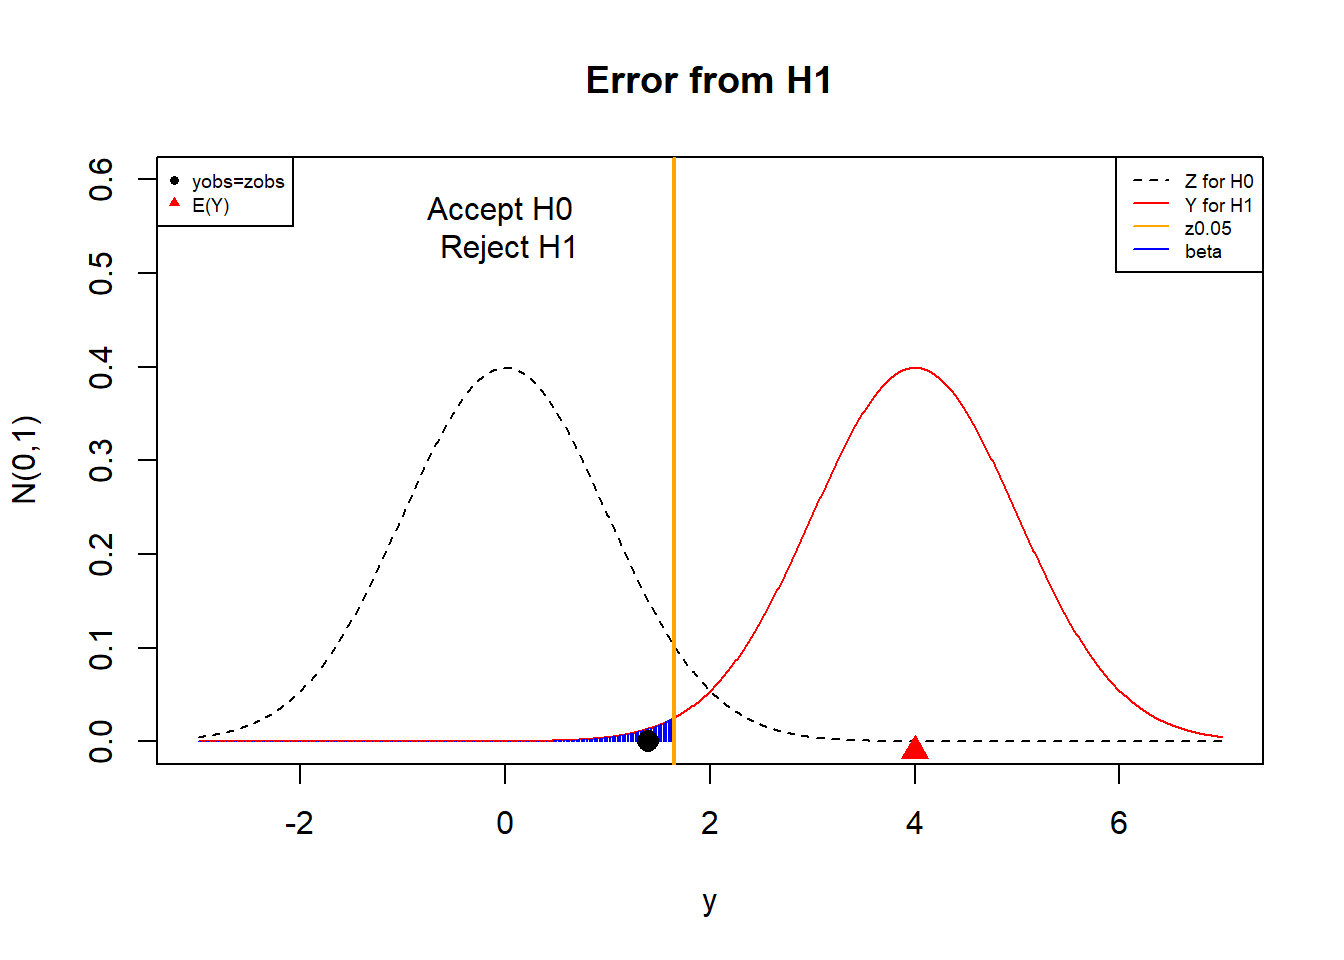
\includegraphics{_main_files/figure-latex/unnamed-chunk-28-1.pdf}
La \textbf{frecuencia relativa} \(f_i=\frac{n_i}{N}\) parece una medida de probabilidad razonable porque

\begin{itemize}
\tightlist
\item
  es un número entre \(0\) y \(1\).
\item
  mide la proporción del total de observaciones que observamos de un resultado particular.
\end{itemize}

Como \(f_{12}=0.25\) entonces estaríamos un cuarto seguros, una de cada 4 observaciones, de obtener \(12\).

\textbf{Pregunta}: ¿Qué tan bueno es \(f_i\) como medida de certeza del resultado \(i\)?

\textbf{Ejemplo (experimento aleatorio con mas repeticiones)}

Digamos que repetimos el experimento 100000 veces más:

La tabla de frecuencias es ahora

\begin{verbatim}
##    outcome    ni      fi
## 1        2  2807 0.02807
## 2        3  5607 0.05607
## 3        4  8435 0.08435
## 4        5 11070 0.11070
## 5        6 13940 0.13940
## 6        7 16613 0.16613
## 7        8 13806 0.13806
## 8        9 10962 0.10962
## 9       10  8402 0.08402
## 10      11  5581 0.05581
## 11      12  2777 0.02777
\end{verbatim}

y el gráfico de barras es

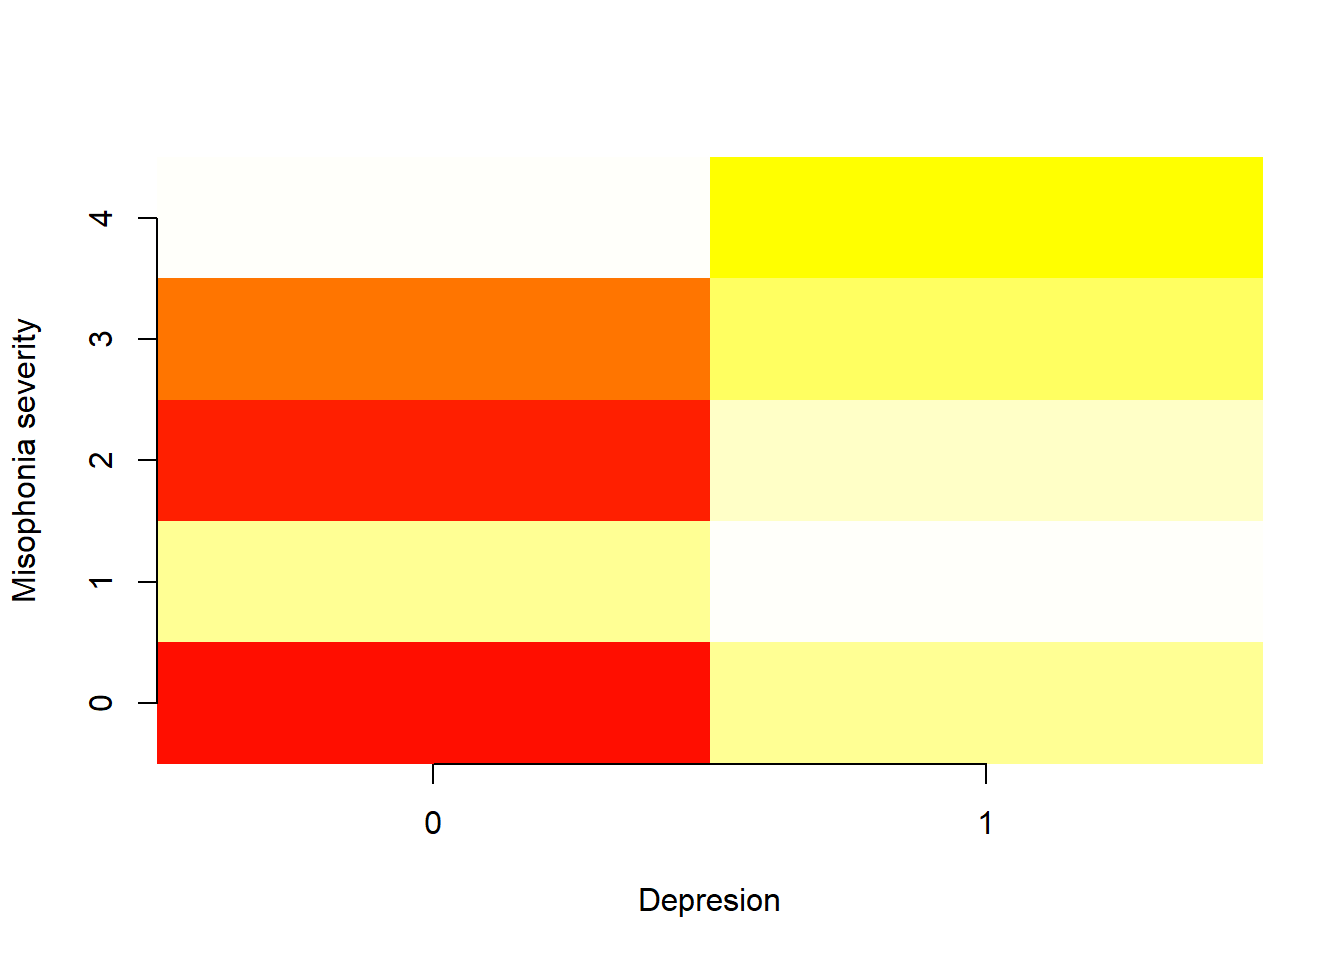
\includegraphics{_main_files/figure-latex/unnamed-chunk-30-1.pdf}

Aparecieron nuevos resultados y \(f_{12}\) ahora es solo \(0.027\), y entonces estamos sólo un \(\sim 3\%\) seguros de obtener \(12\) en el próximo experimento. Las probabilidades medidas por \(f_i\) cambian con \(N\).

\hypertarget{frecuencias-relativas-en-el-infinito}{%
\section{Frecuencias relativas en el infinito}\label{frecuencias-relativas-en-el-infinito}}

Una observación crucial es que si medimos las probabilidades de \(f_i\) en valores crecientes de \(N\) ¡\textbf{convergen}!

En este gráfico cada sección vertical da la frecuencia relativa de cada observación. Vemos que después de \(N=1000\) (\(log10(N)=3\)) las proporciones apenas varían con mas \(N\).

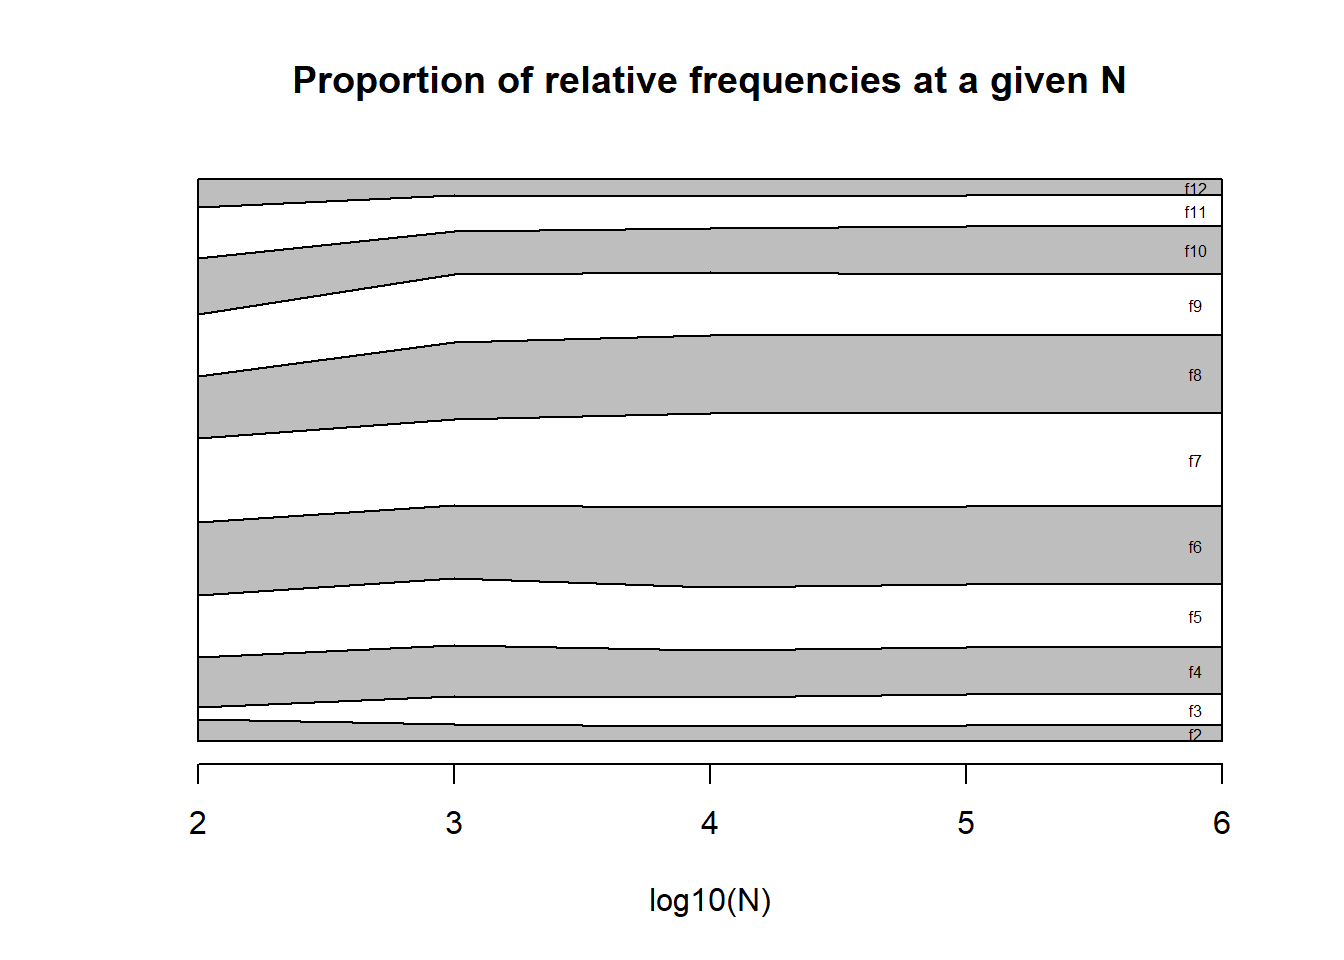
\includegraphics{_main_files/figure-latex/unnamed-chunk-31-1.pdf}
Encontramos que cada una de las frecuencias relativas \(f_i\) converge a un valor constante

\[lim_{N\rightarrow \infty} f_i = P_i\]

\hypertarget{probabilidad-frecuentista}{%
\section{Probabilidad frecuentista}\label{probabilidad-frecuentista}}

Llamamos \textbf{Probabilidad} \(P_i\) al límite cuando \(N \rightarrow \infty\) de la \textbf{frecuencia relativa} de observar el resultado \(i\) en un experimento aleatorio.

Defendida por Venn (1876), la definición frecuentista de probabilidad se deriva de datos/experiencia (empírica).

\begin{itemize}
\tightlist
\item
  No observamos \(P_i\), observamos \(f_i\)
\item
  \textbf{Estimamos} \(P_i\) con \(f_i\) (normalmente cuando \(N\) es grande), escribimos: \[\hat{P_i}=f_i\]
\end{itemize}

Similar a la relación entre \textbf{observación} y \textbf{resultado}, tenemos la relación entre \textbf{frecuencia relativa} y \textbf{probabilidad} como un valor concreto de una cantidad abstracta.

\hypertarget{probabilidades-cluxe1sicas-y-frecuentistas}{%
\section{Probabilidades clásicas y frecuentistas}\label{probabilidades-cluxe1sicas-y-frecuentistas}}

Tenemos situaciones en las que se puede usar la probabilidad clásica para encontrar el límite de frecuencias relativas.

\begin{itemize}
\tightlist
\item
  Si los resultados son \textbf{igualmente probables}, la probabilidad clásica nos da el límite:
\end{itemize}

\[P_i=lim_{N\rightarrow \infty} \frac{n_i}{N}=\frac{1}{M}\]

\begin{itemize}
\tightlist
\item
  Si los resultados en los que estamos interesados pueden derivarse de otros resultados \textbf{igualmente probables}; Veremos más sobre esto cuando estudiemos los modelos de probabilidad.
\end{itemize}

\textbf{Ejemplo (suma de dos dados)}

Nuestro ejemplo anterior se basa en la \textbf{suma de dos dados}.
Si bien realizamos el experimento muchas veces, anotamos los resultados y calculamos las \textbf{frecuencias relativas}, podemos conocer el valor exacto de probabilidad.

Esta probabilidad \textbf{se deduce} del hecho de que el resultado de cada dado es \textbf{igualmente probable}. A partir de esta suposición, podemos encontrar que (Ejercicio 1)

\[
    P_i= 
\begin{cases}
   \frac{i-1}{36},& i \in \{2,3,4,5,6, 7\} \\
\frac{13-i}{36},& i \in \{8,9,10,11,12\} \\ 
\end{cases}
\]

La motivación de la definición frecuentista es \textbf{empírica} (datos) mientras que la de la definición clásica es \textbf{racional} (modelos). A menudo combinamos ambos enfoques (inferencia y deducción) para conocer las probabilidades de nuestro experimento aleatorio.

\hypertarget{definiciuxf3n-de-probabilidad}{%
\section{Definición de probabilidad}\label{definiciuxf3n-de-probabilidad}}

Una probabilidad es un número que se asigna a cada resultado posible de un experimento aleatorio y satisface las siguientes propiedades o \textbf{axiomas}:

\begin{enumerate}
\def\labelenumi{\arabic{enumi})}
\tightlist
\item
  cuando los resultados \(E_1\) y \(E_2\) son mutuamente excluyentes; es decir, solo uno de ellos puede ocurrir, entonces la probabilidad de observar \(E_1\) \textbf{o} \(E_1\), escrito como \(E_1\cup E_2\), es su suma:
  \[P(E_1\cup E_2) = P(E_1) + P(E_2)\]
\item
  cuando \(S\) es el conjunto de todos los resultados posibles, entonces su probabilidad es \(1\) (al menos se observa algo): \[P(S)=1\]
\item
  La probabilidad de cualquier resultado está entre 0 y 1 \[P(E) \in [0,1]\]
\end{enumerate}

Propuesto por Kolmogorov's hace menos de 100 años (1933)

\hypertarget{tabla-de-probabilidades}{%
\section{Tabla de probabilidades}\label{tabla-de-probabilidades}}

Las propiedades de Kolmogorov son las reglas básicas para construir una \textbf{tabla de probabilidad}, de manera similar a la tabla de frecuencia relativa.

\textbf{Ejemplo (Dado)}

La tabla de probabilidad para el lanzamiento de un dado

\begin{longtable}[]{@{}cc@{}}
\toprule
resultado & Probabilidad \\
\midrule
\endhead
\(1\) & 1/6 \\
\(2\) & 1/6 \\
\(3\) & 1/6 \\
\(4\) & 1/6 \\
\(5\) & 1/6 \\
\(6\) & 1/6 \\
\(P(1 \cup 2\cup ... \cup 6)\) & 1 \\
\bottomrule
\end{longtable}

Verifiquemos los axiomas:

\begin{enumerate}
\def\labelenumi{\arabic{enumi})}
\item
  Donde \(1 \cup 2\) es, por ejemplo, el \textbf{evento} de lanzar un \(1\) \textbf{o} un \(2\). Entonces \[P(1 \cup 2)=P(1)+P(2)=2/6\]
\item
  Como \(S=\{1,2,3,4,5,6\}\) se compone de resultados \textbf{mutuamente excluyentes}, entonces
\end{enumerate}

\[P(S)=P(1\cup 2\cup ... \cup 6) = P(1)+P(2)+ ...+P(n)=1\]

\begin{enumerate}
\def\labelenumi{\arabic{enumi})}
\setcounter{enumi}{2}
\tightlist
\item
  Las probabilidades de cada uno de resultados están entre \(0\) y \(1\).
\end{enumerate}

\hypertarget{espacio-muestral}{%
\section{Espacio muestral}\label{espacio-muestral}}

El conjunto de todos los resultados posibles de un experimento aleatorio se denomina \textbf{espacio muestral} y se denota como \(S\).

El espacio muestral puede estar formado por resultados categóricos o numéricos.

\emph{Por ejemplo:}

\begin{itemize}
\tightlist
\item
  temperatura humana: \(S = (36, 42)\) grados Celsius.
\item
  niveles de azúcar en humanos: \(S=(70-80) mg/dL\)
\item
  el tamaño de un tornillo de una línea de producción: \(S=(70-72) mm\)
\item
  número de correos electrónicos recibidos en una hora: \(S =\{1, ...\infty \}\)
\item
  el lanzamiento de un dado: \(S=\{1, 2, 3, 4, 5, 6\}\)
\end{itemize}

\hypertarget{eventos}{%
\section{Eventos}\label{eventos}}

Un \textbf{evento} \(A\) es un \textbf{subconjunto} del espacio muestral. Es una \textbf{colección} de resultados.

\emph{Ejemplos de eventos:}

\begin{itemize}
\tightlist
\item
  El evento de una temperatura saludable: \(A=37-38\) grados Celsius
\item
  El evento de producir un tornillo con un tamaño: \(A=71.5mm\)
\item
  El evento de recibir más de 4 emails en una hora: \(A=\{4, \infty \}\)
\item
  El evento de obtener un número menor o igual a 3 en la tirada de a dice: \(A=\{1,2,3\}\)
\end{itemize}

Un evento se refiere a un posible conjunto de \textbf{resultados}.

\hypertarget{uxe1lgebra-de-eventos}{%
\section{Álgebra de eventos}\label{uxe1lgebra-de-eventos}}

Para dos eventos \(A\) y \(B\), podemos construir los siguientes eventos derivados utilizando las operaciones básicas de conjuntos:

\begin{itemize}
\tightlist
\item
  Complemento \(A'\): el evento de \textbf{no} \(A\)
\item
  Unión \(A \cup B\): el evento de \(A\) \textbf{o} \(B\)
\item
  Intersección \(A \cap B\): el evento de \(A\) \textbf{y} \(B\)
\end{itemize}

\textbf{Ejemplo (dado)}

Lancemos un dado y veamos los eventos (conjunto de resultados):

\begin{itemize}
\tightlist
\item
  un número menor o igual a tres \(A:\{1,2,3\}\)
\item
  un número par \(B:\{2,4,6\}\)
\end{itemize}

Veamos como podemos construir nuevos eventos con las operaciones de conjuntos:

\begin{itemize}
\tightlist
\item
  un número no menor de tres: \(A':\{4,5,6\}\)
\item
  un número menor o igual a tres \textbf{o} par: \(A \cup B: \{1,2,3,4,6\}\)
\item
  un número menor o igual a tres \textbf{y} par \(A \cap B: \{2\}\)
\end{itemize}

\hypertarget{resultados-mutuamente-excluyentes}{%
\section{Resultados mutuamente excluyentes}\label{resultados-mutuamente-excluyentes}}

Los resultados como tirar \(1\) y \(2\) en un dado son eventos que no pueden ocurrir al mismo tiempo. Decimos que son \textbf{mutuamente excluyentes}.

En general, dos eventos denotados como \(E_1\) y \(E_2\) son mutuamente excluyentes cuando

\[E_1\cap E_2=\emptyset\]

\emph{Ejemplos:}

\begin{itemize}
\item
  El resultado de tener una gravedad de misofonía de \(1\) y una gravedad de \(4\).
\item
  Los resultados de obtener \(12\) y \(5\) al sumar el lanzamiento de dos dados.
\end{itemize}

De acuerdo con las propiedades de Kolmogorov, solo los resultados \textbf{mutuamente excluyentes} se pueden organizar en \textbf{tablas de probabilidad}, como en las tablas de frecuencias relativas.

\hypertarget{probabilidades-conjuntas}{%
\section{Probabilidades conjuntas}\label{probabilidades-conjuntas}}

La \textbf{probabilidad conjunta} de \(A\) y \(B\) es la probabilidad de \(A\) y \(B\). Eso es \[P(A \cap B)\] o \(P(A,B)\).

Para escribir probabilidades conjuntas de eventos no mutuamente excluyentes (\(A \cap B \neq \emptyset\)) en una tabla de probabilidad, notamos que siempre podemos descomponer el espacio muestral en conjuntos \textbf{mutuamente excluyentes} que involucran las intersecciones:

\(S=\{A\cap B, A \cap B', A'\cap B, A'\cap B'\}\)

\textbf{Consideremos el diagrama de Ven} para el ejemplo donde \(A\) es el evento que corresponde a sacar número menor o igual que 3 y \(B\) corresponde a un número par:

Las \textbf{marginales} de \(A\) y \(B\) son la probabilidad de \(A\) y la probabilidad de \(B\), respectivamente:

\begin{itemize}
\tightlist
\item
  \(P(A)=P(A\cap B') + P(A \cap B)=2/6+1/6=3/6\)
\item
  \(P(B)=P(A'\cap B) +P(A \cap B)=2/6+1/6=3/6\)
\end{itemize}

Podemos ahora escribir la \textbf{tabla de probabilidad} para las probabilidades conjuntas

\begin{longtable}[]{@{}cc@{}}
\toprule
Resultado & Probabilidad \\
\midrule
\endhead
\((A \cap B)\) & \(P(A \cap B)=1/6\) \\
\((A\cap B')\) & \(P(A \cap B')=2/6\) \\
\((A' \cap B)\) & \(P(A' \cap B)=2/6\) \\
\((A' \cap B')\) & \(P(A' \cap B')=1/6\) \\
suma & \(1\) \\
\bottomrule
\end{longtable}

Cada resultado tiene \(dos\) valores (uno para la característica del tipo \(A\) y otro para el tipo \(B\))

\hypertarget{tabla-de-contingencia}{%
\section{Tabla de contingencia}\label{tabla-de-contingencia}}

La tabla de probabilidad conjunta también se puede escribir en una \textbf{tabla de contingencia}

\begin{longtable}[]{@{}cccc@{}}
\toprule
& \(B\) & \(B'\) & suma \\
\midrule
\endhead
\(A\) & \(P(A \cap B )\) & \(P(A\cap B' )\) & \(P(A)\) \\
\(A'\) & \(P(A'\cap B )\) & \(P(A'\cap B' )\) & \(P(A')\) \\
suma & \(P(B)\) & \(P(B')\) & 1 \\
\bottomrule
\end{longtable}

Donde las marginales son las sumas en las márgenes de la tabla, por ejemplo:

\begin{itemize}
\tightlist
\item
  \(P(A)=P(A \cap B') + P(A \cap B)\)
\item
  \(P(B)=P(A' \cap B) +P(A \cap B)\)
\end{itemize}

En nuestro ejemplo, la tabla de contingencia es

\begin{longtable}[]{@{}cccc@{}}
\toprule
& \(B\) & \(B'\) & suma \\
\midrule
\endhead
\(A\) & \(1/6\) & \(2/6\) & \(3/6\) \\
\(A'\) & \(2/6\) & \(1/6\) & \(3/6\) \\
suma & \(3/6\) & \(3/6\) & 1 \\
\bottomrule
\end{longtable}

\hypertarget{la-regla-de-la-suma}{%
\section{La regla de la suma:}\label{la-regla-de-la-suma}}

La regla de la suma nos permite calcular la probabilidad de \(A\) o \(B\), \(P(A \cup B)\), en términos de la probabilidad de \(A\) y \(B\), \(P(A \cap B)\). Podemos hacer esto de tres maneras equivalentes:

\begin{enumerate}
\def\labelenumi{\arabic{enumi})}
\item
  Usando las marginales y la probabilidad conjunta
  \[P(A \cup B)=P(A) + P(B) - P(A\cap B)\]
\item
  Usando solo probabilidades conjuntas
  \[P(A \cup B)=P(A \cap B)+P(A\cap B')+P(A'\cap B)\]
\item
  Usando el complemento de la probabilidad conjunta
  \[P(A \cup B)=1-P(A'\cap B')\]
\end{enumerate}

\textbf{Ejemplo (dado)}

Tomemos los eventos \(A:\{1,2,3\}\), sacar un número menor o igual que \(3\), y \(B:\{2,4,6\}\), sacar un número par en el lanzamiento de un dado.

Por lo tanto:

\begin{enumerate}
\def\labelenumi{\arabic{enumi})}
\item
  \(P(A \cup B)=P(A) + P(B) - P(A\cap B)=3/6+3/6-1/6=5/6\)
\item
  \(P(A \cup B)=P(A \cap B)+P(A\cap B')+P(A'\cap B)=1/6+2/6+2/6=5/6\)
\item
  \(P(A \cup B)=1-P(A'\cap B')= 1-1/6=5/6\)
\end{enumerate}

En la tabla de contingencia \(P(A \cup B)\) corresponde a las casillas en negrita (o sea todas menos 1/6 de abajo a la derecha)

\begin{longtable}[]{@{}ccc@{}}
\toprule
& \(B\) & \(B'\) \\
\midrule
\endhead
\(A\) & \textbf{1/6} & \textbf{2/6} \\
\(A'\) & \textbf{2/6} & 1/6 \\
\bottomrule
\end{longtable}

\hypertarget{preguntas-1}{%
\section{Preguntas}\label{preguntas-1}}

Recopilamos la edad y categoría de 100 deportistas en una competición

\begin{longtable}[]{@{}ccc@{}}
\toprule
& \(edad:junior\) & \(edad:senior\) \\
\midrule
\endhead
\(categoria:1ra\) & \(14\) & \(12\) \\
\(categoria:2a\) & \(21\) & \(18\) \\
\(categoria:3a\) & \(22\) & \(13\) \\
\bottomrule
\end{longtable}

\textbf{1)} ¿Cuál es la probabilidad estimada de que un deportista sea de 2ª categoría y senior?

\textbf{\(\qquad\)a:} \(18/100\); \textbf{\(\qquad\)b:} \(18/43\); \textbf{\(\qquad\)c:} \(18\); \textbf{\(\qquad\)d:} \(18/39\)

\textbf{2)} ¿Cuál es la probabilidad estimada de que el atleta no esté en la tercera categoría y sea senior?

\textbf{\(\qquad\)a:} \(35/100\); \textbf{\(\qquad\)b:} \(30/100\); \textbf{\(\qquad\)c:} \(22/100\); \textbf{\(\qquad\)d:} \(13/100\)

\textbf{3)} ¿Cuál es la probabilidad marginal de la tercera categoría?

\textbf{\(\qquad\)a:} \(13/100\); \textbf{\(\qquad\)b:} \(35/100\); \textbf{\(\qquad\)c:} \(22/100\); \textbf{\(\qquad\)d:} \(13/22\)

\textbf{4)} ¿Cuál es la probabilidad marginal de ser senior?

\textbf{\(\qquad\)a:} \(13/100\); \textbf{\(\qquad\)b:} \(43/100\); \textbf{\(\qquad\)c:} \(43/57\); \textbf{\(\qquad\)d:} \(57/100\)

\textbf{5)} ¿Cuál es la probabilidad de ser senior o de tercera categoría?

\textbf{\(\qquad\)a:} \(65/100\); \textbf{\(\qquad\)b:} \(86/100\); \textbf{\(\qquad\)c:} \(78/100\); \textbf{\(\qquad\)d:} \(13/100\)

\hypertarget{ejercicios-1}{%
\section{Ejercicios}\label{ejercicios-1}}

\hypertarget{probabilidad-cluxe1sica-ejercicio-1}{%
\subsubsection{Probabilidad clásica: Ejercicio 1}\label{probabilidad-cluxe1sica-ejercicio-1}}

\begin{itemize}
\item
  Escribe la tabla de \textbf{probabilidad conjunta} para los \textbf{resultados} de lanzar dos dados; en las filas escribe los resultados del primer dado y en las columnas los resultados del segundo dado.
\item
  ¿Cuál es la probabilidad de sacar \((3,4)\)? (R:1/36)
\item
  ¿Cuál es la probabilidad de tirar \(3\) y \(4\) con cualquiera de los dos dados? (R:2/36)
\item
  ¿Cuál es la probabilidad de tirar \(3\) en el primer dado o \(4\) en el segundo? (A:11/36)
\item
  ¿Cuál es la probabilidad de tirar \(3\) o \(4\) con cualquier dado? (R:20/36)
\item
  Escribe la \textbf{tabla de probabilidad} para el resultado de la \textbf{suma} de dos dados. Supon que el resultado de cada dado es \textbf{igualmente probable}. Verifica que es:
\end{itemize}

\[
    P_i= 
\begin{cases}
   \frac{i-1}{36},& i \in \{2,3,4,5,6, 7\} \\
\frac{13-i}{36},& i \in \{8,9,10,11,12\} \\ 
\end{cases}
\]

\hypertarget{probabilidad-frecuentista-ejercicio-2}{%
\subsubsection{Probabilidad frecuentista: Ejercicio 2}\label{probabilidad-frecuentista-ejercicio-2}}

El resultado de un experimento aleatorio es medir la gravedad de la misofonía \textbf{y} el estado de depresión de un paciente.

\begin{itemize}
\tightlist
\item
  Gravedad de la misofonía: \(S_M:\{M_0,M_1,M_2,M_3,M_4\}\)
\item
  Depresión: \(S_D:\{D', D\}\))
\end{itemize}

Escribe la tabla de contingencia para las frecuencias absolutas (\(n_{M,D}\)) para un estudio sobre un total de 123 pacientes en el que se observó

\begin{itemize}
\tightlist
\item
  100 individuos no tuvieron depresión.
\item
  Ningún individuo con misofonía 4 y sin depresión.
\item
  5 individuos con misofonía de grado 1 y sin depresión.
\item
  El mismo número que el caso anterior para individuos con depresión y sin misofonía.
\item
  25 individuos sin depresión y grado 3 de misofonía.
\item
  El número de misofónicos sin depresión para los grados 2 y 0 se repartieron a cantiaddes iguales.
\item
  El número de individuos con depresión y misofonía incrementó progresivamente
  en múltiplos de tres, empezando en 0 individuos para grado 1.
\end{itemize}

Reponde las siguientes preguntas:

\begin{itemize}
\tightlist
\item
  ¿Cuantos individuos tuvieron misofonía? (R:83)
\item
  ¿Cuantos individuos tuvieron misofonía de grado 3? (R:31)
\item
  ¿Cuantos individuos tuvieron misofonía de grado 2 sin depresión? (R:35)
\end{itemize}

Escribe las tabla de consingencia para frecuencias relativas \(f_{M,D}\). Supongamos que \(N\) es grande y que las frecuencias absolutas \textbf{estiman} las probabilidades \(f_{M,D}=\hat{P}(M \cap D)\). Responde las siguientes preguntas:

\begin{itemize}
\tightlist
\item
  ¿Cuál es la probabilidad marginal de misofonía de gravedad 2? (R: 0.3)
\item
  ¿Cuál es la probabilidad de no ser misofónico \textbf{y} no estar deprimido? (R:0.284)
\item
  ¿Cuál es la probabilidad de ser misofónico \textbf{o} estar deprimido? (R: 0.715)
\item
  ¿Cuál es la probabilidad de ser misofónico \textbf{y} estar deprimido? (R: 0.146)
\item
  Describir en lenguaje hablado los resultados con probabilidad 0.
\end{itemize}

\hypertarget{ejercicio-3}{%
\subsubsection{Ejercicio 3}\label{ejercicio-3}}

Hemos realizado un experimento aleatorio \(10\) veces, que consiste en anotar el sexo y el estado vital de pacientes con algún tipo de cáncer después de 10 años del diagnóstico. Obtuvimos los siguientes resultados

\begin{verbatim}
##         A     B
## 1    male  dead
## 2    male  dead
## 3    male  dead
## 4  female alive
## 5    male  dead
## 6  female alive
## 7  female  dead
## 8  female alive
## 9    male alive
## 10   male alive
\end{verbatim}

\begin{itemize}
\tightlist
\item
  Crea la tabla de contingencia para el número (\(n_{i,j}\)) de observaciones de cada resultado (\(A,B\))
\item
  Crea la tabla de contingencia para la frecuencia relativa (\(f_{i,j}\)) de los resultados
\item
  ¿Cuál es la frecuencia marginal de ser hombre? (R/0.6)
\item
  ¿Cuál es la frecuencia marginal de estar vivo? (R/0.5)
\item
  ¿Cuál es la frecuencia de estar vivo \textbf{o} ser mujer? (R/0.6)
\end{itemize}

\hypertarget{teoruxeda-ejercicio-4}{%
\subsubsection{Teoría: Ejercicio 4}\label{teoruxeda-ejercicio-4}}

\begin{itemize}
\item
  De la segunda forma de la regla de la suma, obtener la primera y la tercera forma.
\item
  ¿Cuál es la regla de la suma de la tercera forma para la probabilidad de tres eventos \(P(A \cup B \cup C)\)?
\end{itemize}

\hypertarget{probabilidad-condicional}{%
\chapter{Probabilidad condicional}\label{probabilidad-condicional}}

En este capítulo, introduciremos la probabilidad condicional.

Usaremos la probabilidad condicional para definir la independencia estadística.

Discutiremos el teorema de Bayes y discutiremos una de sus principales aplicaciones, que es la eficacia de predicción de una herramienta de diagnóstico.

\hypertarget{probabilidad-conjunta}{%
\section{Probabilidad conjunta}\label{probabilidad-conjunta}}

Recordemos que la probabilidad conjunta de dos eventos \(A\) y \(B\) se define como su intersección

\[P( A,B )=P(A \cap B)\]

Ahora, imagina experimentos aleatorios que miden dos tipos diferentes de resultados.

\begin{itemize}
\item
  altura y peso de un individuo: \((h, w)\)
\item
  tiempo y posición de una carga eléctrica: \((p, t)\)
\item
  el lanzamiento de dos dados: (\(n_1\),\(n_2\))
\item
  cruzar dos semáforos en verde: (\(\bar{R_ 1}\) , \(\bar{R_2}\))
\end{itemize}

A menudo nos interesa saber si los valores de un resultado \textbf{condicionan} los valores del otro.

\hypertarget{independencia-estaduxedstica}{%
\section{Independencia estadística}\label{independencia-estaduxedstica}}

En muchos casos, estamos interesados en saber si dos eventos a menudo tienden a ocurrir juntos. Queremos poder discernir entre dos casos.

\begin{itemize}
\item
  \textbf{Independencia} entre eventos. Por ejemplo, sacar un 1 en un dado no hace más probable sacar otro 1 en un segundo dado.
\item
  \textbf{Correlación} entre eventos. Por ejemplo, si un hombre es alto, probablemente sea pesado.
\end{itemize}

\textbf{Ejemplo (conductor)}

Realizamos un experimento para averiguar si observar fallas estructurales en un material afecta su conductividad.

Los datos se verían como

\begin{longtable}[]{@{}ccc@{}}
\toprule
Director de orquesta & Estructura & Conductividad \\
\midrule
\endhead
\(c_1\) & con fallas & defectuosa \\
\(c_2\) & sin fallas & sin defectos \\
\(c_3\) & con fallas & defectuosa \\
\ldots{} & \ldots{} & \ldots{} \\
\(c_i\) & sin fallas & defectuosa* \\
\ldots{} & \ldots{} & \ldots{} \\
\ldots{} & \ldots{} & \ldots{} \\
\(c_n\) & con fallas & sin defectos* \\
\bottomrule
\end{longtable}

Podemos esperar que la conductividad defectuosa ocurra más a menudo con fallas que sin fallas si las fallas afectan la conductividad.

Imaginemos que a partir de los datos obtenemos la siguiente tabla de contingencia de \textbf{probabilidades conjuntas} estimadas

\begin{longtable}[]{@{}cccc@{}}
\toprule
& con fallas (F) & sin fallas (F') & suma \\
\midrule
\endhead
defectuoso (D) & \(0.005\) & \(0.045\) & \(0.05\) \\
sin defectos (D') & \(0.095\) & \(0.855\) & \(0.95\) \\
suma & \(0.1\) & \(0.9\) & 1 \\
\bottomrule
\end{longtable}

donde, por ejemplo, la probabilidad conjunta de \(F\) y \(D\) es

\begin{itemize}
\tightlist
\item
  \(P(D,F)=0.005\)
\end{itemize}

y las probabilidades marginales son

\begin{itemize}
\tightlist
\item
  \(P(D)=P(D, F) + P(D, F')=0.05\)
\item
  \(P(F)=P(D, F) + P(D', F)= 0.1\).
\end{itemize}

\hypertarget{la-probabilidad-condicional}{%
\section{La probabilidad condicional}\label{la-probabilidad-condicional}}

La conductividad defectuosa es \textbf{independiente} de tener fallas estructurales en el material si la probabilidad de tener conductividad defectuosa (\(D\)) es la misma \textbf{ya sea} que tenga fallas (\(F\)) o no (\(F'\)) .

Consideremos primero solamente los materiales que tienen fallas.

Dentro de aquellos materiales que tienen fallas (\(F\)), ¿cuál es la probabilidad estimada de que sean defectuosos?

\(\hat{P}(D|F)=\frac{n_{F,D}}{n_{F}}=\frac{n_{F,D}/n}{n_{F}/n}= \frac{f_{F,D}}{f_{F}}\)
\[= \frac{\hat{P}(F,D)}{\hat{P}(F)}\]
Por lo tanto, en el límite cuando \(N \rightarrow \infty\), tenemos

\[P(D|F)=\frac{P(F, D)}{P(D)}=\frac{P(F \cap D)}{P(D)}\]
\textbf{Definición:}

La \emph{probabilidad condicional} de un evento \(B\) dado un evento \(A\), indicado como \(P(A|B)\), es
\[P(A|B) = \frac{P(A\cap B)}{P(B)}\]
Podemos probar que la probabilidad condicional satisface los axiomas de probabilidad. La probabilidad condicional se puede entender como una probabilidad con un espacio muestral dado por \(B\): \(S_B\). En nuestro ejemplo, los materiales con fallas.

\hypertarget{tabla-de-contingencia-condicional}{%
\section{Tabla de contingencia condicional}\label{tabla-de-contingencia-condicional}}

Si dividimos las columnas de la tabla de probabilidad conjunta por las probabilidades marginales de los efectos condicionantes (\(F\) y \(F'\)), podemos escribir \textbf{una tabla de contingencia condicional}

\begin{longtable}[]{@{}ccc@{}}
\toprule
& F & F' \\
\midrule
\endhead
D & P(D {\textbar{}} F) & P(D {\textbar{}} F') \\
D' & P(D' {\textbar{}} F) & P(D' {\textbar{}} F') \\
suma & 1 & 1 \\
\bottomrule
\end{longtable}

Donde las probabilidades por columnas suman uno. La primera columna muestra las probabilidades de ser defectuoso o no solo de que los materiales que tienen fallas (primera condición: \(F\)). La segunda columna muestra las probabilidades solo para los materiales que no tienen fallas (segunda condición: \(F'\)).

Las probabilidades condicionales son las probabilidades del evento dentro de cada condición. Las leemos como:

\begin{itemize}
\item
  \(P(D|F)\): Probabilidad de tener conductividad defectuosa \textbf{si} tiene fallas
\item
  \(P(D'|F)\): Probabilidad de no tener conductividad defectuosa \textbf{si} tiene fallas
\item
  \(P(D|F')\): Probabilidad de tener conductividad defectuosa \textbf{si} no tiene fallas
\item
  \(P(D'|F')\) Probabilidad de no tener conductividad defectuosa \textbf{si} no tiene fallas
\end{itemize}

\hypertarget{independencia-estaduxedstica-1}{%
\section{Independencia estadística}\label{independencia-estaduxedstica-1}}

En nuestro ejemplo, la tabla de contingencia condicional es

\begin{longtable}[]{@{}ccc@{}}
\toprule
& F & F' \\
\midrule
\endhead
D & P(D{\textbar{}}F) = 0.05 & P(D{\textbar{}}F')=0.05 \\
D' & P(D'{\textbar{}}F)=0.95 & P(D'{\textbar{}}F')=0.95 \\
suma & 1 & 1 \\
\bottomrule
\end{longtable}

¡Observamos que las probabilidades marginales y condicionales son las mismas!

\begin{itemize}
\tightlist
\item
  \(P(D|F)=P(D|F')=P(D)\)
\item
  \(P(D'|F)=P(D'|F')=P(D')\)
\end{itemize}

Esto quiere decir que la probabilidad de observar un conductor defectuoso \textbf{no} depende tener una falla estructural o no.

Concluimos que la conductividad defectuosa no se ve afectada por tener una falla estructural.

\textbf{Definición}

Dos eventos \(A\) y \(B\) son estadísticamente independientes si ocurre cualquiera de los casos equivalentes

\begin{enumerate}
\def\labelenumi{\arabic{enumi})}
\tightlist
\item
  \(P(A|B)=P(A)\); \(A\) es independiente de \(B\)
\item
  \(P(B|A)=P(B)\); \(B\) es independiente de \(A\)
\end{enumerate}

y por la definición de probabilidad condicional

\begin{enumerate}
\def\labelenumi{\arabic{enumi})}
\setcounter{enumi}{2}
\tightlist
\item
  \(P(A\cap B)=P(A|B)P(B)=P(A)P(B)\)
\end{enumerate}

Esta tercera forma es un enunciado sobre las probabilidades conjuntas. Dice que podemos obtener probabilidades conjuntas por la multiplicación de las marginales.

En nuestra tabla de probabilidad conjunta original

\begin{longtable}[]{@{}cccc@{}}
\toprule
& F & F' & suma \\
\midrule
\endhead
D & \(0.005\) & \(0.045\) & \(0.05\) \\
D' & \(0.095\) & \(0.855\) & \(0.95\) \\
suma & \(0.1\) & \(0.9\) & 1 \\
\bottomrule
\end{longtable}

podemos confirmar que todas las entradas de la matriz son el producto de las marginales. Por ejemplo: \(P(F)P(D)= P(D \cap F)\) y \(P(D')P(F')=P(D' \cap F')\). Por lo tanto, ser defectuoso es independiente de tener un defecto.

\textbf{Ejemplo (Monedas)}

Queremos confirmar que los resultados de lanzar dos monedas son independientes. Consideramos que todos los resultados son igualmente probables:

\begin{longtable}[]{@{}cc@{}}
\toprule
resultado & Probabilidad \\
\midrule
\endhead
\((H,T)\) & 1/4 \\
\((H,H)\) & 1/4 \\
\((T,T)\) & 1/4 \\
\((T,H)\) & 1/4 \\
suma & 1 \\
\bottomrule
\end{longtable}

donde \((H,T)\) es, por ejemplo, el evento de cara en la primera moneda y cruz en la segunda moneda. La tabla de contingencia para las probabilidades conjuntas es:

\begin{longtable}[]{@{}cccc@{}}
\toprule
& H & T & suma \\
\midrule
\endhead
H & \(1/4\) & \(1/4\) & \(1/2\) \\
T & \(1/4\) & \(1/4\) & \(1/2\) \\
suma & \(1/2\) & \(1/2\) & 1 \\
\bottomrule
\end{longtable}

De esta tabla vemos que la probabilidad de obtener una cara y luego una cruz es el producto de las marginales \(P(H, T)=P(H)*P(T)=1/4\). Por lo tanto, el evento de cara en la primera moneda y cruz en la segunda son independientes.

Si elaboramos la tabla de contingencia condicional sobre el lanzamiento de la primera moneda veremos que obtener cruz en la segunda moneda no está condicionado por haber obtenido cara en la primera moneda: \(P(T|H)=P(T) =1/2\)

\hypertarget{dependencia-estaduxedstica}{%
\section{Dependencia estadística}\label{dependencia-estaduxedstica}}

Un ejemplo importante de dependencia estadística se encuentra en el desempeño de \textbf{herramientas de diagnóstico}, donde queremos determinar el estado de un sistema (s) con resultados

\begin{itemize}
\tightlist
\item
  inadecuado (si)
\item
  adecuado (no)
\end{itemize}

con una prueba (t) con resultados

\begin{itemize}
\tightlist
\item
  positivo
\item
  negativo
\end{itemize}

Por ejemplo, probamos una batería para saber cuánto tiempo puede durar. Tensamos un cable para saber si resiste llevar cierta carga. Realizamos una PCR para ver si alguien está infectado.

\hypertarget{prueba-de-diagnuxf3stico}{%
\section{Prueba de diagnóstico}\label{prueba-de-diagnuxf3stico}}

Consideremos diagnosticar una infección con una nueva prueba. Estado de infección:

\begin{itemize}
\tightlist
\item
  si (infectado)
\item
  no (no infectado)
\end{itemize}

Prueba:

\begin{itemize}
\tightlist
\item
  positivo
\item
  negativo
\end{itemize}

La \textbf{tabla de contingencia condicional} es lo que obtenemos en un ambiente controlado (laboratorio)

\begin{longtable}[]{@{}ccc@{}}
\toprule
& Infección: si & Infección: No \\
\midrule
\endhead
Test: positivo & P(positivo {\textbar{}} si) & P(positivo {\textbar{}} no) \\
Test: negativo & P(negativo {\textbar{}} si) & P(negativo {\textbar{}} no) \\
suma & 1 & 1 \\
\bottomrule
\end{longtable}

Miremos las entradas de la tabla
1) Tasa de verdaderos positivos (Sensibilidad): La probabilidad de dar positivo \textbf{si} tiene la enfermedad \(P(positivo|si)\)

\begin{enumerate}
\def\labelenumi{\arabic{enumi})}
\setcounter{enumi}{1}
\item
  Tasa de verdaderos negativos (Especificidad): La probabilidad de dar negativo \textbf{si} no tiene la enfermedad \(P(negativo|no)\)
\item
  Tasa de falsos positivos: la probabilidad de dar positivo \textbf{si} no tiene la enfermedad \(P(positivo|no)\)
\item
  Tasa de falsos negativos: la probabilidad de dar negativo \textbf{si} tiene la enfermedad \(P(negativo|si)\)
\end{enumerate}

Alta correlación (dependencia estadística) entre la prueba y la infección significa valores altos de las probabilidades 1 y 2 \textbf{y} valores bajos para las probabilidades 3 y 4.

\textbf{Ejemplo (COVID)}

Ahora consideremos una situación real. En los días iniciales de la pandemia de coronavirus no había una medida de la eficacia de las PCR para detectar el virus. Uno de los primeros estudios publicados (\url{https://www.nejm.org/doi/full/10.1056/NEJMp2015897}) encontró que

\begin{itemize}
\tightlist
\item
  Las PCR tuvieron una sensibilidad del 70\%, en condición de infección.
\item
  Las PCR tuvieron una especificidad del 94\%, en condición de no infección.
\end{itemize}

La tabla de contingencia condicional es

\begin{longtable}[]{@{}ccc@{}}
\toprule
& Infección: si & Infección: No \\
\midrule
\endhead
Test: positivo & P(positivo{\textbar{}}si)=0.7 & P(positivo{\textbar{}}no)=0.06 \\
Test: negativo & P(negativo{\textbar{}}si)=0.3 & P(negativo{\textbar{}}no)=0.94 \\
suma & 1 & 1 \\
\bottomrule
\end{longtable}

Por lo tanto, los errores en las pruebas de diagnóstico fueron:

\begin{itemize}
\tightlist
\item
  La tasa de falsos positivos es \(P(positivo|no)=0.06\)
\item
  La tasa de falsos negativos es \(P(negativo|si)=0.3\)
\end{itemize}

\hypertarget{probabilidades-inversas}{%
\section{Probabilidades inversas}\label{probabilidades-inversas}}

Nos interesa encontrar la probabilidad de estar infectado si la prueba da positivo: \[P(si|positivo)\]

Para eso:

\begin{enumerate}
\def\labelenumi{\arabic{enumi}.}
\tightlist
\item
  Recuperamos la tabla de contingencia para probabilidades conjuntas, multiplicando por las marginales
\end{enumerate}

\begin{longtable}[]{@{}cccc@{}}
\toprule
& Infección: si & Infección: No & suma \\
\midrule
\endhead
Test: positivo & P(positivo {\textbar{}} si)P(si) & P(positivo {\textbar{}} no)P(no) & P(positivo) \\
Test: negativo & P(negativo {\textbar{}} si)P(si) & P(negativo {\textbar{}} no) P(no) & P(negativo) \\
suma & P(si) & P(no) & 1 \\
\bottomrule
\end{longtable}

\begin{enumerate}
\def\labelenumi{\arabic{enumi}.}
\setcounter{enumi}{1}
\tightlist
\item
  Usamos la definición de probabilidades condicionales para filas en lugar de columnas (dividimos por la marginal de los resultados de la prueba)
\end{enumerate}

\begin{longtable}[]{@{}cccc@{}}
\toprule
& Infección: si & Infección: No & suma \\
\midrule
\endhead
Test: positivo & P(si{\textbar{}}positivo) & P(sin{\textbar{}}positivo) & 1 \\
Test: negativo & P(si{\textbar{}}negativo) & P(sin{\textbar{}}negativo) & 1 \\
\bottomrule
\end{longtable}

Por ejemplo:

\[P(si|positivo)=\frac{P(positivo|si)P(si)}{P(positivo)}\]

Para aplicar esta fórmula necesitamos las marginales \(P(si)\) (incidencia) y \(P(positivo)\).

\begin{itemize}
\item
  Para encontrar \(P(si)\), necesitamos un nuevo estudio: el primer estudio de prevalencia en España mostró que durante el confinamiento \(P(si)=0.05\), \(P(no)=0.95\), antes del verano de 2020.
\item
  Para encontrar \(P(positivo)\), podemos usar la definición de probabilidad marginal y condicional:
\end{itemize}

\(P(positivo)=P(positivo \cap si) + P(positivo \cap no)\)
\[= P(positivo|si)P(si)+P(positivo|no)P(no)\]
Esta última relación de las marginales se llama \textbf{regla de probabilidad total}.

\hypertarget{teorema-de-bayes}{%
\section{Teorema de Bayes}\label{teorema-de-bayes}}

Después de sustituir la regla de probabilidad total en \(P(si|positivo)\), tenemos

\[P(si|positivo)=\frac{P(positivo|si)P(si)}{P(positivo|si)P(si)+P(positivo|no)P(no)}\]
Esta expresión se conoce como \textbf{teorema de Bayes}. Nos permite invertir los condicionales:

\[P(positivo|si) \rightarrow P(si|positivo)\]
O \textbf{evaluar} una prueba en una condición controlada (infección) y luego usarla para \textbf{inferir} la probabilidad de la condición cuando la prueba es positiva.

\textbf{Ejemplo (COVID)}:

El rendimiento de la prueba fue:

\begin{itemize}
\item
  Sensibilidad: \(P(positivo|si)=0.70\)
\item
  Tasa de falsos positivos: \(P(positivo|no)=1- P(negativo|no)=0.06\)
\end{itemize}

El estudio en población española dio:

\begin{itemize}
\tightlist
\item
  \(P(si)=0.05\)
\item
  \(P(no)=1-P(si)=0.95\).
\end{itemize}

Por lo tanto, la probabilidad de estar infectado en caso de dar positivo era:

\[P(si|positivo)=0.38\]

Concluimos que en ese momento las PCR no eran muy buenas para \textbf{confirmar} infecciones.

Sin embargo, apliquemos ahora el teorema de Bayes a la probabilidad de no estar infectado si la prueba fue negativa.

\[P(no|negativo) = \frac{P(negativo|no) P(no)}{P(negativo|no) P(no)+P(negativo|si)P(si)}\]

La sustitución de todos los valores da

\[P(no|negativo)=0.98\]

Por lo tanto, las pruebas eran buenas para \textbf{descartar} infecciones y un requisito justo para viajar.

\textbf{Teorema de Bayes}

En general, podemos tener más de dos eventos condicionantes. Por lo tanto, el teorema de Baye dice:

Si \(E1, E2, ..., Ek\) son \(k\) eventos mutuamente excluyentes y exhaustivos y \(B\) es cualquier evento, entonces la probabilidad inversa \(P(Ei|B)\) es

\[P(Ei|B)=\frac{P(B|Ei)P(Ei)}{P(B|E1)P(E1) +...+ P(B|Ek)P(Ek)} \]
El denominador es la regla de probabilidad total para la marginal \(P(B)\), en términos de las marginales \(P(E1), P(E2), ... P(Ek)\).

\[P(B)=P(B|E1)P(E1) +...+ P(B|Ek)P(Ek)\]

\textbf{Árbol condicional}

La regla de probabilidad total también se puede ilustrar usando un árbol \textbf{condicional}.

\textbf{Regla de probabilidad total} para la marginal de \(B\): ¿De cuántas maneras puedo obtener el resultado \(B\)?

\(P(B)=P(B|A)P(A)+P(B|A')P(A')\)

\hypertarget{ejercicios-2}{%
\section{Ejercicios}\label{ejercicios-2}}

\hypertarget{preguntas-2}{%
\section{Preguntas}\label{preguntas-2}}

Recopilamos la edad y categoría de 100 deportistas en una competición

\begin{longtable}[]{@{}ccc@{}}
\toprule
& \(junior\) & \(senior\) \\
\midrule
\endhead
\(1er\) & \(14\) & \(12\) \\
\(2do\) & \(21\) & \(18\) \\
\(3er\) & \(22\) & \(13\) \\
\bottomrule
\end{longtable}

\textbf{1)} ¿Cuál es la probabilidad estimada de que el atleta esté en la tercera categoría si el atleta es junior?

\textbf{\(\qquad\)a:} \(22\); \textbf{\(\qquad\)b:} \(22/100\); \textbf{\(\qquad\)c:} \(22/57\); \textbf{\(\qquad\)d:} \(22/35\);

\textbf{2)} ¿Cuál es la probabilidad estimada de que el atleta sea junior y esté en 1ra categoría si el atleta no está en 3ra categoría?

\textbf{\(\qquad\)a:} \(14/35\); \textbf{\(\qquad\)b:} \(14/65\); \textbf{\(\qquad\)c:} \(14/100\); \textbf{\(\qquad\)d:} \(14/26\)

\textbf{3)} Una prueba diagnóstica tiene una probabilidad de \(8/9\) de detectar una enfermedad si los pacientes están enfermos y una probabilidad de \(3/9\) de detectar la enfermedad si los pacientes están sanos. Si la probabilidad de estar enfermo es \(1/9\). ¿Cuál es la probabilidad de que un paciente esté enfermo si una prueba detecta la enfermedad?

\textbf{\(\qquad\)a:} \(\frac{8/9}{8/9+3/9}*1/9\); \textbf{\(\qquad\)b:} \(\frac{3/9}{8/9+3/9}*1/9\); \textbf{\(\qquad\)c:} \(\frac{3/9*8/9}{8/9*1/9+3/9*8/9}\); \textbf{\(\qquad\)d:} \(\frac{8/9*1/9}{8/9*1/9+3/9*8/9}\);

\textbf{4)} Como se comenta en las notas, una prueba PCR para coronavirus tenía una sensibilidad del 70 \% y una especificidad del 94 \% y en España durante el confinamiento hubo una incidencia del 5 \%. Con estos datos, ¿cuál era la probabilidad de dar positivo en España (\(P(positivo)\))

\textbf{\(\qquad\)a:} \(0.035\); \textbf{\(\qquad\)b:} \(0.092\); \textbf{\(\qquad\)c:} \(0.908\); \textbf{\(\qquad\)d:} \(0.95\)

\textbf{5)} Con los mismos datos que en la pregunta 4, dar positivo en la PCR y estar infectado no son eventos independientes porque:

\textbf{\(\qquad\)a:} La sensibilidad es del 70\%; \textbf{\(\qquad\)b:} La sensibilidad y la tasa de falsos positivos son diferentes; \textbf{\(\qquad\)c:} La tasa de falsos positivos es del 0.06\%; \textbf{\(\qquad\)d:} la especificidad es del 96\%

\hypertarget{ejercicio-1-1}{%
\subsubsection{Ejercicio 1}\label{ejercicio-1-1}}

Se prueba el rendimiento de una máquina para producir varillas de torneado de alta calidad. Estos son los resultados de las pruebas

\begin{longtable}[]{@{}ccc@{}}
\toprule
& Redondeado: si & Redondeado: No \\
\midrule
\endhead
superficie lisa: si & 200 & 1 \\
superficie lisa: no & 4 & 2 \\
\bottomrule
\end{longtable}

\begin{itemize}
\item
  ¿Cuál es la probabilidad estimada de que la máquina produzca una varilla que no satisfaga ningún control de calidad? (R: 2/207)
\item
  ¿Cuál es la probabilidad estimada de que la máquina produzca una varilla que no satisfaga al menos un control de calidad? (R: 7/207)
\item
  ¿Cuál es la probabilidad estimada de que la máquina produzca varillas de superficie redondeada y alisada? (R: 200/207)
\item
  ¿Cuál es la probabilidad estimada de que la barra sea redondeada si la barra es lisa? (R: 200/201)
\item
  ¿Cuál es la probabilidad estimada de que la varilla sea lisa si es redondeada? (R: 200/204)
\item
  ¿Cuál es la probabilidad estimada de que la varilla no sea ni lisa ni redondeada si no satisface al menos un control de calidad? (R: 2/7)
\item
  ¿Son eventos independientes la lisa y la redondez? (No)
\end{itemize}

\hypertarget{ejercicio-2-1}{%
\subsubsection{Ejercicio 2}\label{ejercicio-2-1}}

Desarrollamos un test para detectar la presencia de bacterias en un lago. Encontramos que si el lago contiene la bacteria, la prueba es positiva el 70\% de las veces. Si no hay bacterias, la prueba es negativa el 60\% de las veces. Implementamos la prueba en una región donde sabemos que el 20\% de los lagos tienen bacterias.

\begin{itemize}
\tightlist
\item
  ¿Cuál es la probabilidad de que un lago que dé positivo esté contaminado con bacterias? (R: 0.30)
\end{itemize}

\hypertarget{ejercicio-3-1}{%
\subsubsection{Ejercicio 3}\label{ejercicio-3-1}}

Se prueba el rendimiento de dos máquinas para producir varillas de torneado de alta calidad. Estos son los resultados de las pruebas

\textbf{Máquina 1}

\begin{longtable}[]{@{}ccc@{}}
\toprule
& Redondeado: si & Redondeado: No \\
\midrule
\endhead
superficie lisa: si & 200 & 1 \\
superficie lisa: no & 4 & 2 \\
\bottomrule
\end{longtable}

\textbf{Máquina 2}

\begin{longtable}[]{@{}ccc@{}}
\toprule
& Redondeado: si & Redondeado: No \\
\midrule
\endhead
superficie lisa: si & 145 & 4 \\
superficie lisa: no & 8 & 6 \\
\bottomrule
\end{longtable}

\begin{itemize}
\tightlist
\item
  ¿Cuál es la probabilidad de que la barra sea redondeada? (R: 357/370)
\item
  ¿Cuál es la probabilidad de que la varilla haya sido producida por la máquina 1? (R: 207/370)
\item
  ¿Cuál es la probabilidad de que la varilla no sea lisa? (R: 20/370)
\item
  ¿Cuál es la probabilidad de que la varilla sea lisa o redondeada o producida por la máquina 1? (R: 364/370)
\item
  ¿Cuál es la probabilidad de que la varilla quede redondeada si es alisada y de la máquina 1? (R: 200/201)
\item
  ¿Cuál es la probabilidad de que la varilla no esté redondeada si no está alisada y es de la máquina 2? (R: 6/8)
\item
  ¿Cuál es la probabilidad de que la varilla haya salido de la máquina 1 si está alisada y redondeada? (R: 200/345)
\item
  ¿Cuál es la probabilidad de que la varilla haya venido de la máquina 2 si no pasa al menos uno de los controles de calidad? (R:0.72)
\end{itemize}

\hypertarget{ejercicio-4}{%
\subsubsection{Ejercicio 4}\label{ejercicio-4}}

Queremos cruzar una avenida con dos semáforos. La probabilidad de encontrar el primer semáforo en rojo es 0.6. Si paramos en el primer semáforo, la probabilidad de parar en el segundo es 0.15. Mientras que la probabilidad de detenernos en el segundo si no nos detenemos en el primero es 0.25.

Cuando intentamos cruzar ambos semáforos:

\begin{itemize}
\tightlist
\item
  ¿Cuál es la probabilidad de tener que detenerse en cada semáforo? (R:0.09)
\item
  ¿Cuál es la probabilidad de tener que parar en al menos un semáforo? (R:0.7)
\item
  ¿Cuál es la probabilidad de tener que detenerse en un solo semáforo? (R:0.61)
\item
  Si paré en el segundo semáforo, ¿cuál es la probabilidad de que tuviera que parar en el primero? (R: 0.47)
\item
  Si tuviera que parar en cualquier semáforo, ¿cuál es la probabilidad de que tuviera que hacerlo dos veces? (R: 0.12)
\item
  ¿Parar en el primer semáforo es un evento independiente de detenerse en el segundo semáforo? (No)
\end{itemize}

Ahora, queremos cruzar una avenida con tres semáforos. La probabilidad de encontrar un semáforo en rojo solo depende de la anterior. En concreto, la probabilidad de encontrar un semáforo en rojo dado que el anterior estaba en rojo es de 0.15. Mientras que la probabilidad de encontrar un tráfico justo en rojo dado que el anterior estaba en verde es de 0.25. Además, la probabilidad de encontrar el primer semáforo en rojo es de 0.6.

\begin{itemize}
\tightlist
\item
  ¿Cuál es la probabilidad de tener que parar en cada semáforo? (R:0.013)
\item
  ¿Cuál es la probabilidad de tener que parar en al menos un semáforo? (R:0.775)
\item
  ¿Cuál es la probabilidad de tener que detenerse en un solo semáforo? (R:0.5425)
\end{itemize}

consejos:

\begin{itemize}
\item
  Si la probabilidad de que un semáforo esté en rojo depende únicamente del anterior, entonces
  \(P(R_3|R_2,R_1)=P(R_3|R_2,\bar{R}_1)=P(R_3|R_2)\) y \(P(R_3|\bar{R}_2,R_1)=P(R_3 |\bar{R}_2,\bar{R}_1)=P(R_3|\bar{R}_2)\)
\item
  La probabilidad conjunta de encontrar tres semáforos en rojo se puede escribir como:
  \(P(R_1,R_2,R_3)=P(R_3|R_2)P(R_2|R_1)P(R_1)\)
\end{itemize}

\hypertarget{ejercicio-5}{%
\subsubsection{Ejercicio 5}\label{ejercicio-5}}

Una prueba de calidad en un ladrillo aleatorio se define por los eventos:

\begin{itemize}
\tightlist
\item
  Pasar la prueba de calidad: \(E\), no pasar la prueba de calidad: \(\bar{E}\)
\item
  Defectuoso: \(D\), no defectuoso: \(\bar{D}\)
\end{itemize}

Si la prueba diagnóstica tiene sensibilidad \(P(E|\bar{D})=0.99\) y especificidad \(P(\bar{E}|D)=0.98\), y la probabilidad de pasar la prueba es \(P(E) =0.893\) entonces

\begin{itemize}
\item
  ¿Cuál es la probabilidad de que un ladrillo elegido al azar sea defectuoso \(P(D)\)? (R:0.1)
\item
  ¿Cuál es la probabilidad de que un ladrillo que ha pasado la prueba sea realmente defectuoso? (R:0.022)
\item
  La probabilidad de que un ladrillo no sea defectuoso \textbf{y} que no pase la prueba (R:0.009)
\item
  ¿Son \(D\) y \(\bar{E}\) estadísticamente independientes? (No)
\end{itemize}

  \bibliography{book.bib,packages.bib}

\end{document}
